\documentclass[10pt]{report}
\usepackage[utf8]{inputenc}

\usepackage{graphicx}
\usepackage{geometry}
\usepackage{enumitem}
\usepackage{hyperref}
\usepackage{colortbl}
\usepackage{array}
\usepackage{float}
\usepackage{tabularx}
\usepackage{longtable}
\usepackage{xcolor}
\usepackage{tikz}
\usepackage{aeguill}
\usepackage{vcell}
\definecolor{plantucolor0000}{RGB}{255,255,255}
\definecolor{plantucolor0001}{RGB}{0,0,0}

\hypersetup{
    colorlinks=true,
    linkcolor=blue,
    filecolor=magenta,      
    urlcolor=cyan,
    pdftitle={Requirement Analysis and Specification Document},}

\graphicspath{ {Images/} }
\geometry{a4paper, margin=100px}

\title{Design Document}
% https://github.com/AndreaPrati98/MaccarronePellizzerPrati
\author{Maccarrone Salvatore,   Pellizzer Massimiliano,   Prati Andrea}
\date{\today}

\begin{document}

% Title Page
% ----------------------------------------------------------------------------------------------------
\begin{titlepage}
    \begin{figure}[t]
        \centering
        
\includegraphics[width=250px]{/PolimiLogo}
    \end{figure}
    \begin{centering}
       \maketitle
    \end{centering}
\end{titlepage}

% ----------------------------------------------------------------------------------------------------

\tableofcontents

\chapter{Introduction}
Agriculture plays a pivotal role in India’s economy. Climate change continues to be a real and potent threat to the agriculture sector, which will impact everything from productivity to livelihoods across food and farm systems and is predicted to result in a 4\%-26\% loss in net farm income towards the end of the century. This calls for a revamp of the entire mechanism that brings food from farms to our plates. The COVID-19 pandemic has greatly highlighted the massive disruption caused in food supply chains exposing the vulnerabilities of marginalized communities, small holder farmers and the importance of building resilient food systems. It has become even more important now that we develop and adopt innovative methodologies and technologies that can help bolster countries against food supply shocks and challenges.

    \section{Purpose}
    Telangana’s government wants to design, develop and demonstrate anticipatory governance models for food systems using digital public goods and community-centric approaches to strengthen data-driven policy making in the state. This will require the involvement of multiple stakeholders, from normal citizens to policy makers, farmers, market analysts, agronomists and so on. \\ \\
    In the first place, Telangana wants to partner with IT providers with the aim of acquiring and combining: \\ 
    Data concerning meteorological short-term and long-term forecasts. Telangana already collects and makes available such data (see https://www.tsdps.telangana.gov.in/aws.jsp).
    \begin{itemize}
    \item Information provided by the farmers about their production (types of products, produced amount per product). 
    \item Information obtained by the water irrigation system concerning the amount of water used by each farmer. 
    \item Information obtained by sensors deployed on the territory and measuring the humidity of soil.
    \item Information obtained by the governmental agronomists who periodically visit the farms in their areas.
    \end{itemize}
    Acquiring and combining such data, DREAM will support the work of three types of actors: policy makers, farmers, and agronomists. In the following we describe the goals summed up.

    \subsection{Goals}
    \subsubsection{G1 - Data-Driven approach}
    \emph{DREAM} will be able to fetch data from different databases. Then, DREAM will be able to collect, analyze and perform inference on this data in order to extract new knowledge that will be at the service of different \emph{DREAM}’s users.
    \subsubsection{G2 - Help policy makers to implement better policies which will make Telangana’s agriculture better}
    \emph{DREAM} will allow policy makers to see real time data regarding Telangana and Telangana’s farms. In particular they will be able to see which farms are performing well and which farms are performing poorly. Moreover, they will be able to understand which steering initiatives are working and which not.
    \subsubsection{G3 - Help farmers to become weather resilient and increase their production}
    \emph{DREAM} will allow farmers to see statistics regarding their farms. Moreover, \emph{DREAM} will provide to them personalized suggestions based on the data regarding their farm and on the data regarding farms that are doing particularly well in similar environments.
    \subsubsection{G4 - Facilitate and make systematic the communication between farmers and agronomists}
    \emph{DREAM} will make communications between agronomists and farmers easy and stable. In fact, \emph{DREAM} will allow farmers to chat with agronomists in just a few clicks. Moreover they will be able to request agronomists to visit them when they are facing complex problems.
    Agronomists, instead, will be able to access real time data regarding farms they are responsible for, and therefore they will be able to see which farms are performing well and which farms are performing poorly. Based on this knowledge, agronomists will be able to decide how much and when to visit each farm, and to send periodical reports to policy makers regarding how the farms (they are responsible for) are doing.
    \subsubsection{G5 - Create a network of farmers}
    Through \emph{DREAM}, farmers will be able to communicate between each other in order to exchange best practices and advice.
    \section{Scope}
    The problem that Telangana is facing concerns the world of agriculture, and it has a very important weight on the lives of many people who, due to various impediments mentioned in the previous section, need a platform that can support them and allow those who create support initiatives to do the work in the most scientific way possible, keeping track of how is all going on without losing information. \\ \\
    To reach this goal, called "data-driven approach" it was necessary to think at an entire platform. In particular, this platform can be seen as divided into three categories:
    \begin{itemize}
        \item Data: users must be able to easily interact with the data to which they have the right to access. They are offered different views and aggregations with respect to this data. The available data can include weather forecasts, the state and composition of the land of an area of Telangana, the water irrigation system (the amount of water used), and the initiatives taken by other farmers who have distinguished themselves for being productive considering the conditions in which they were found (positive and negative deviance). Other types of data are described in the remainder of the document.
        \item Community: users are able to communicate via two communication channels within the system, one is the Forum and the other is the Chat System that will allow Farmers and Agronomists to talk to each other to exchange advice and clarifications.
        \item Management: users can organize physical visits between Agronomists and Farmers directly in the app.
    \end{itemize}
    The processing of data and their analysis was not the focus for the drafting of this document. In fact, the first goal was to think about how to develop the platform as a whole. The choice on which criteria to calculate the Farmer's performance (i.e. their deviance, positive or negative) will be made thanks to the collaboration with expert agronomists who will provide all the knowledge to be able to create and study intelligent models using special tools such as, TensorFlow, a framework for processing data. \\
    Moreover, the system will interface itself with different databases maintained and managed by third parties. How the data are inserted or managed in those databases is not one of the concern of the system described in this document.
    \section{Definitions, Acronyms, Abbreviations}
    \subsection{Definitions}
    \emph{Agronomist's schedule} $\rightarrow$ The schedule of an agronomist is a list of planned activities or things to be done showing the times or dates when they are intended to happen or be done. In particular, in this case, the activities are the planned visits to the various farms.
    \\ \\
    \emph{Area} $\rightarrow$ The word "area" indicates a disjoint partition of Telangana. In fact, Telengana is partitioned in several disjoint areas, and to each area are associated both farmers and agronomists, in such a way that:
    \begin{itemize}
        \item Each area can have one or more farmers and one or more agronomists
        \item Each farmer is associated to one and only one area
        \item Each agronomist is associated to one and only one area
    \end{itemize}
    \emph{Chat} $\rightarrow$ A chat is a virtual space that, after it has opened, allows one agronomist and one farmer to discuss with each other.
    \\ \\
    \emph{Data Summary} $\rightarrow$ A data summary is an aggregation of data fetched by various databases, which gives a certain data view of a subject (e.g. a farm or an area).
    \\ \\
    \emph{Data View} $\rightarrow$ A data view is a selection of data fetched by the various databases, regarding a specific aspect (e.g. humidity of soil, water irrigation data) of the subject (e.g. a farm or an area of Telangana).
    \\ \\
    \emph{Priority} $\rightarrow$ The term "priority", when used referring to the list of farms, indicates that the list of farms is sorted taking into account:
    \begin{itemize}
        \item The number of times the farm has already been visited during the year
        \item How well or bad the farm is performing
        \item Possible requests of help done by the farmer
    \end{itemize}
    These metrics define what is referred to as priority.
    \\ \\
    \emph{Relevant data} $\rightarrow$ The term "relevant data" indicates data regarding:
    \begin{itemize}
        \item Data concerning meteorological short-term and long-term forecasts
        \item Information provided by the farmers about their production
        \item Information obtained by the water irrigation system concerning the amount of water used by each farmer
        \item Information obtained by sensors deployed on the territory and measuring the humidity of soil
        \item Information obtained by the governmental agronomists who periodically visit the farms in their areas
    \end{itemize}
    \emph{Report} $\rightarrow$ When an agronomist visits a farm they must write (and insert into the system) a summary of what they have suggested to the farmer, which problems they have detected, and everything they think could be relevant in order to understand why the farmer is performing well or why the farmer is performing poorly. This summary is indicated by the word “report”. The purpose of the report is to keep track of the history of every farm.
    \\ \\
    \emph{Ticket (or Chat Request)} $\rightarrow$ Whenever a farmer wants to have a chat with an agronomist they have to open a ticket. A ticket, thus, is a request to have a chat.
    \\ \\
    \emph{Open a ticket} $\rightarrow$ Open a ticket indicates the action, performed by the farmer, of asking an agronomist to have a chat.
    \\ \\
    \emph{Managed ticket} $\rightarrow$ A managed ticket is a chat request accepted by an agronomist.
    \\ \\
    \emph{Not manged ticket} $\rightarrow$ A ticket that is not managed is a chat request not accepted by any agronomist yet.
    \\ \\
    \emph{Users} $\rightarrow$ The users of the system are: farmers, agronomists and policy makers. Whenever the word "users" is used, it indicates both agronomists, farmers and policy makers.
    \\ \\
    \emph{Visit} $\rightarrow$ In order to help farmers, agronomists can reach the farm of the farmer physically. A visit, therefore, is the action, performed by an agronomist, of physically reaching a farmer's farm.
    \\ \\
    \emph{Booking a visit} $\rightarrow$ To book a visit means reaching an agreement between a farmer and an agronomist on when the agronomist should visit the farm.
    \\ \\
    \emph{Booked visit} $\rightarrow$ A booked visit is a visit that has been scheduled by the agronomist in accordance with the farmer
    \subsection{Acronyms}
    \emph{API} $\rightarrow$ Application Programming Interface, it indicates on demand procedure which supply a specific task.\\ \\
    \emph{BPMN} $\rightarrow$ Business Process Model and Notation, it is a graphical representation for specifying business processes in a business process model.\\ \\
    \emph{DBMS} $\rightarrow$ Data Base Management System, it is an interface between the end user and the database, simultaneously managing the data, the database engine, and the database schema in order to facilitate the organization and manipulation of data.\\ \\
    \emph{DREAM} $\rightarrow$ Data-Drive Predictive Farming in Telengana, is the name software to be developed, described in this document.
    IOT
\section{Revision History}
\section{Reference Documents}
\emph{Multiple Tier Architecture} $\rightarrow$ https://www.ibm.com/cloud/learn/three-tier-architecture\\ \\
\emph{Big Data Architectures} $\rightarrow$ https://docs.microsoft.com/en-us/azure/architecture/data-guide/big-data/\\ \\
\emph{Apache Spark} $\rightarrow$ https://spark.apache.org/
\emph{Reference book} $\rightarrow$ Hans Van Vilet - Software Engineering: Principles and Practice
\emph{Github} $\rightarrow$ https://github.com/UNDP-India/Data4Policy\\ (All the reference written on this repository are reference that we considered as well)
\section{Document Structure}

\chapter{Architectural Design}
\section{Overview: High-Level Components and their interaction}
The system to develop is a distributed application which follows a 4-tier client-server architecture. In particular, the application will be divided in the following tiers:
\begin{enumerate}
    \item Presentation Tier
    \item Application Tier
    \item Data Tier
    \item Big-Data Tier
\end{enumerate}
\begin{figure}[H]
    \centering
    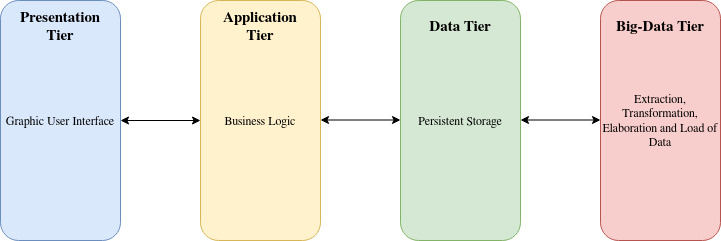
\includegraphics[width=250px]{Architecture/FourTiers_01.jpg}
    \caption{Four-Tier Application (High-Level View)}
\end{figure}
The presentation tier is where the user interface and the communication layer of the application are implemented and where the user interacts with the application. Its main purpose is to display information to the user and collect information from the user. This top-level tier will run both on thin clients as well as thick clients, in fact, the presentation tier software can run both on a web browser, as well as mobile application.
\newline
\newline
The application tier, also known as the logic tier or middle tier, is where information collected in the presentation tier is processed (sometimes against other information in the data tier) using business logic, which means a specific set of business rules. The application tier can also add, delete or modify data in the data tier, in fact, this tier is able to communicate with the data tier by using API calls.
\newline
\newline
The data tier is where the information processed by the application is stored and managed. In particular this tier will contain the DBMS used by the application in order to store and retrieve data.
\newline
\newline
The big-data tier is the tier responsible to automatically fetch data both from, elaborate and store data into the internal database in order to extract valuable knowledge from raw data. In particular this tier will be responsible for automatically fetching data both from the internal database as well as from the third parties' databases (through known API), elaborate those data, and store the results into the internal database.
\newline
\newline
Below is shown the architecture adopted in more detail:
\begin{figure}[H]
    \centering
    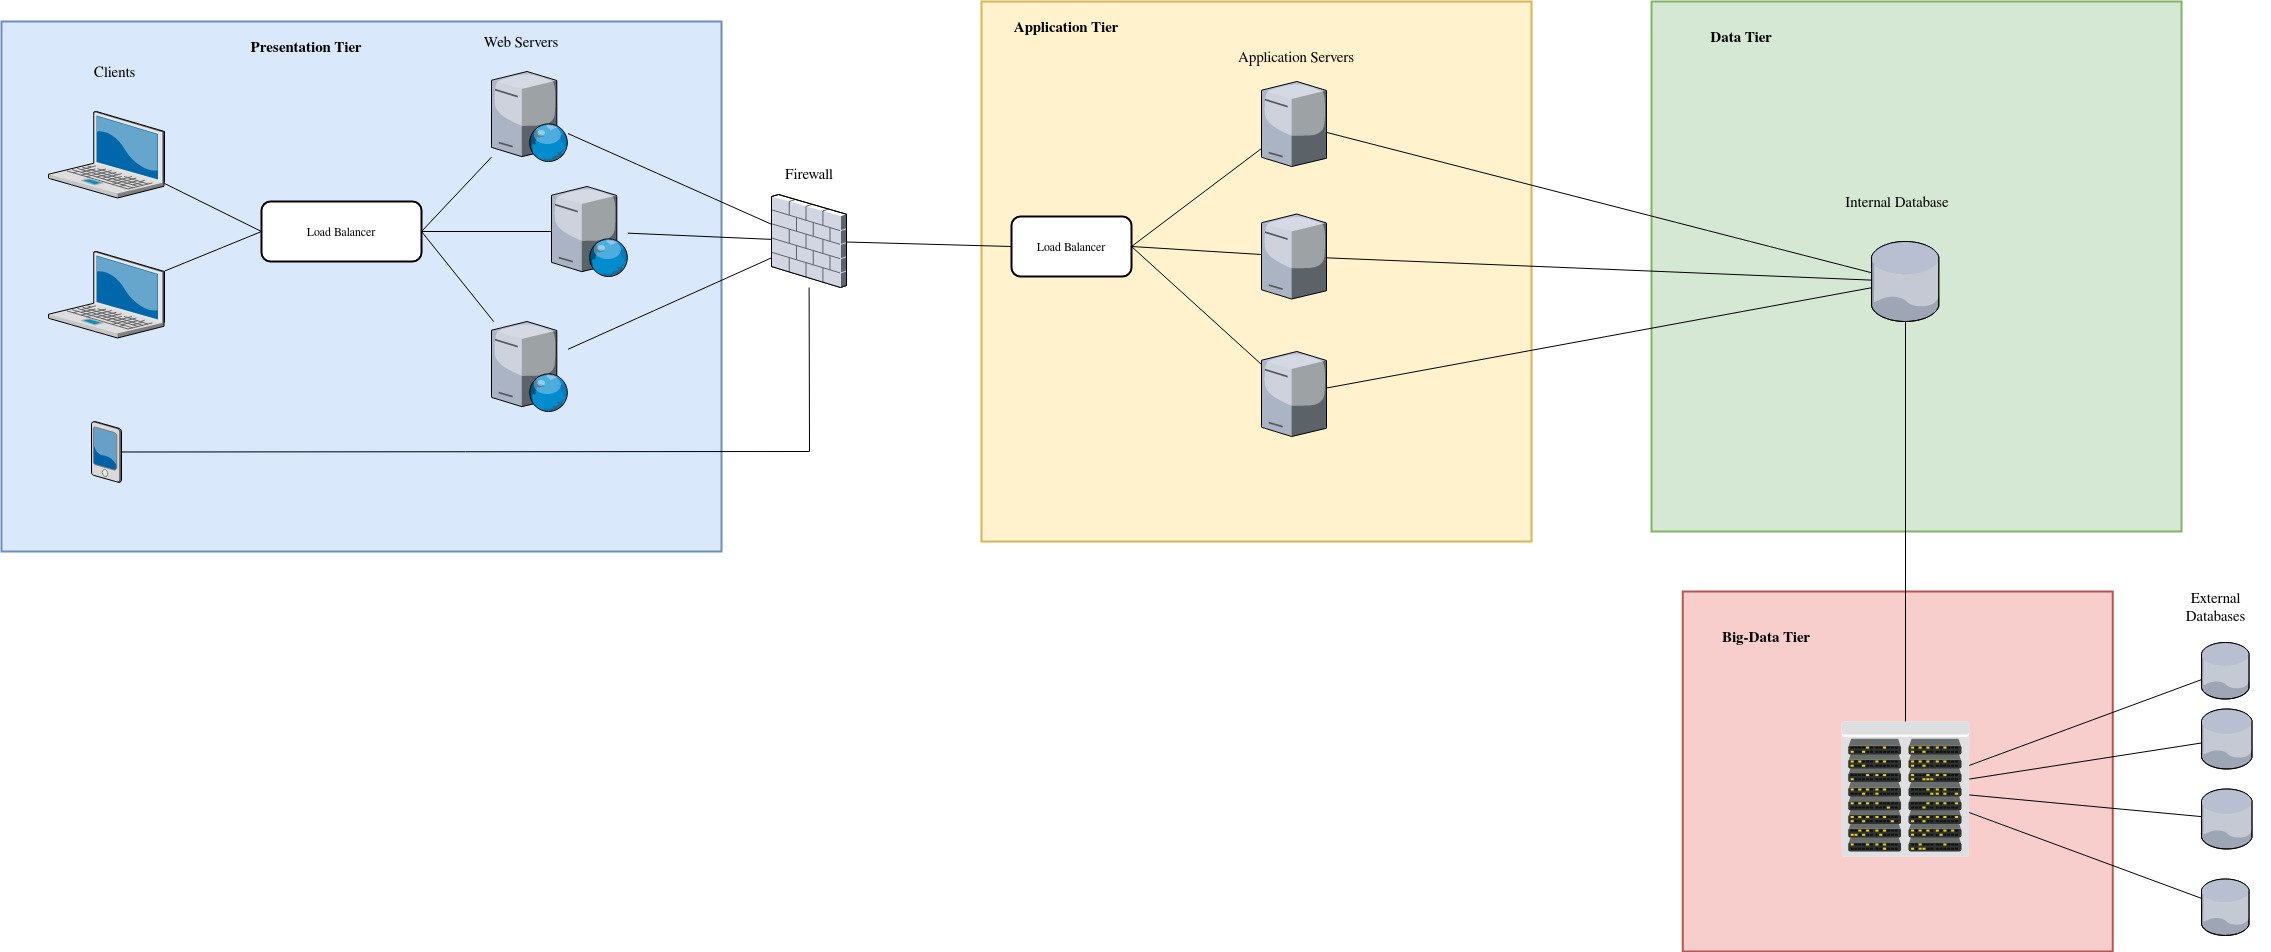
\includegraphics[width=350px]{Architecture/FourTiers_02.jpg}
    \caption{Four-Tier Application (Low-Level View)}
\end{figure}
It is possible to notice that the system is supposed to be accessed through both a web interface and a mobile application, and this is valid for all kinds of users. In particular, those users which use a web browser will communicate with a web server (which, in turn, interfaces itself with the application tier), while, in case of using the mobile application, the core of the software installed on the user’s device will interface with the business layer’s APIs, which send and receive all the information, in order to work properly, directly to the application servers.\\ \\ 
The presentation tier and the application tier is divided by a firewall, for security purposes.\\\ \\
The communications between the presentation tier and the application tier are REST (Representational State Transfer) compliant, which means that:
\begin{itemize}
    \item Interactions are client-server and stateless. This means that the history is not accumulated with time, giving an advantage in term of scalability. Eventually a caching service can be used in order to reduce latency in case the clients send multiple time the same request, avoiding the server to execute multiple time the same functions.
    \item The data within a response to a request must be implicitly or explicitly labeled as cacheable or non-cacheable. The ability of caching data is key to provide scalability.
    \item Each component cannot ”see” beyond the immediate layer which it is interacting with.
    \item Components expose a uniform interface.
\end{itemize}
The application tier, which contains the application's logic, will use an ORM (Object-Relational Mapping) programming technique in order to interface with the DBMS exploiting the advantages of the object-oriented paradigm.\\ \\
It is possible to see that both the web server and the application server can be replicated, in order to manage the high loads without affecting the performance.\\ \\
The data tier, as said before contains the internal database of the system. The internal database will be replicated and distributed, and it will possibly hosted in the cloud.\\ \\
The big-data tier is responsible for fetching data both from internal and external databases, make computations on them, and store the results in the proprietary database. In fact, this tier is responsible for analyzing data, extracting statistics from them, and making inference on them. Given the huge amount of data to process this tier must be hosted in cloud, in order to be scalable and to able to manage higher and higher loads of data. More on this tier will be explained in a dedicated section.

\section{Component View}
\begin{figure}
    \centering
    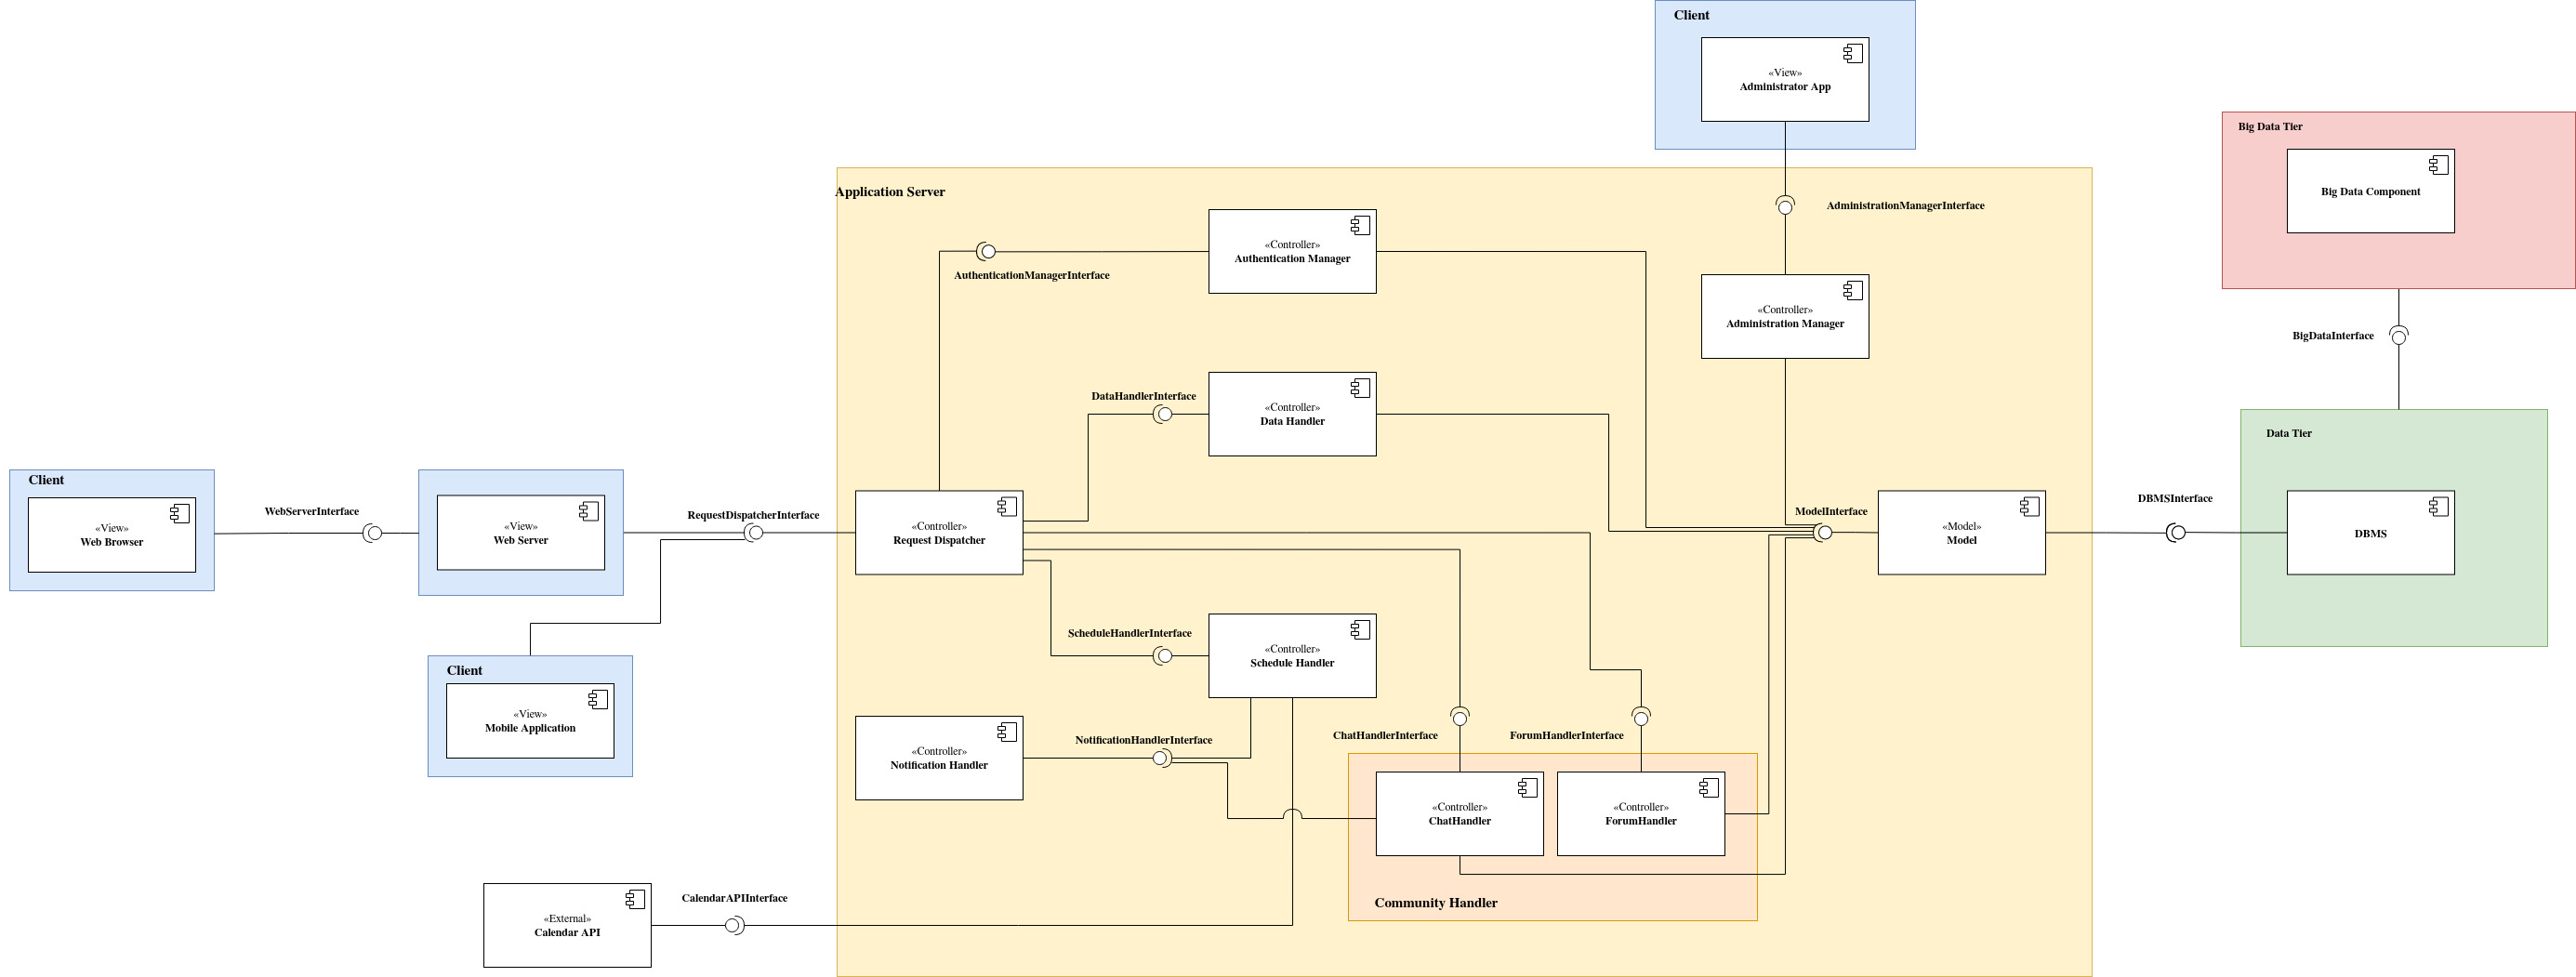
\includegraphics[width=\paperwidth, angle=-90]{Component/ComponentDiagram.jpg}
    \caption{Component Diagram}
    \label{fig:component_diagram}
\end{figure}


This diagram below shows the main components that shape DREAM. As described previously the components are organized in the four-tier architecture: Presentation, Application, Data and Big-Data.\\ Here we will focus on the \textbf{Application Tier}, to describe how data is processed.\\\\
The web browser and the mobile application are the components with which the users can interact with the system. We provided also an Administrator application that is needed to allow sysadmins to maintain and support the system.\\\\
Inside the \textbf{Application server} we have:
\begin{itemize}
    \item \textbf{RequestDispatcher}: it routes the requests to the other components according to the function that the user requires.
    \item \textbf{AuthenticationManager}: it is in charge of the registration and login of the users
    \item \textbf{DataHandler}: it is the component that retrieves, stores and manages data that do not belong to what concerns the Community subsystem. In fact, this component can store reports of visits, retrieve list of farms, and other functionalities that will be depicted in the sequence diagrams, in the following section.
    \item \textbf{ScheduleHandler}: it is the component that handles the schedules of the agronomists in terms of creating, editing and deleting visits. To do so, it has to interact with the NotificationHandler, to manage notification, and with an external component that manages the calendar.
    \item \textbf{NotificationHandler}: it is in charge of sending notification to the users about several events, such as, an upcoming visit, a new pending chat and so on.
\end{itemize}
Then we have the \textbf{Community subsystem}, that has two components:
\begin{itemize}
    \item \textbf{ChatHandler}: it is the component that manages everything related to the functioning of the chats. It interacts with the NotificationHandler to send notifications about the chats, but also with the Model to store data in the DMBS.
    \item \textbf{ForumHandler}: similar to what the ChatHandler does, but applied to the forum. Morevoer, the interaction is with the Model to store data in the DMBS, while forum notifications are not needed at the time this document is written.
\end{itemize}



Finally, the \textbf{Model}: the component of the system that allows every other
component to interact with the chosen DBMS. It represents the
application's dynamic data structure. Notice that, it is independent of the user interface
It directly manages the data, logic, and rules of the application.




\section{Big-Data Tier}
The big data tier was introduced in order to handle the ingestion, processing, and analysis of data that is too large or complex for traditional database systems. This tier, in fact, is responsible for periodically fetching data from the different databases (both the internal one as well as the external ones), transform and elaborate the data in order to extract valuable knowledge from it, and store the results of different computations inside the internal database.
\subsection{Components of the Big Data Tier}
The following diagram shows the logical components that typically fit into a big data tier.
\begin{figure}[H]
    \centering
    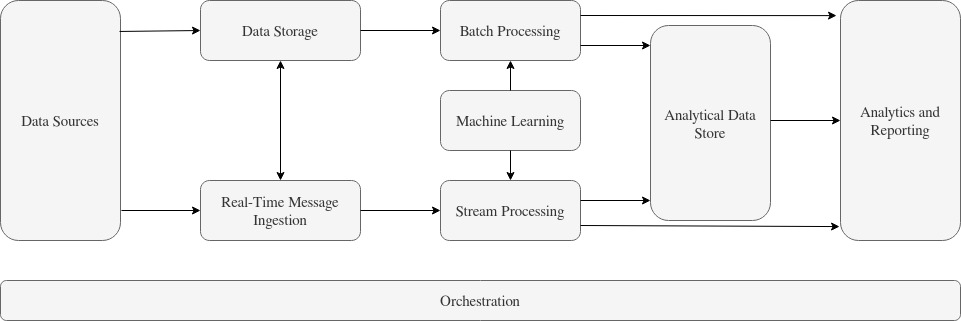
\includegraphics[width=350px]{Architecture/BigDataArchitecture.jpg}
    \caption{Generic Big Data Architecture Components}
\end{figure}
Here there is a brief description of each component:
\begin{itemize}
    \item \emph{Data Sources} They are the various sources from witch the system extracts data. They could be relational databases, static files produced by the application, as well as real time data sources, such as IoT devices.
    \item \emph{Data Storage} This component is a distributed file store that can hold high volumes of large files in various formats. It is used in order to store data for batch processing operations.
    \item \emph{Batch Processing} Often a big data solution must process data files using long-running batch jobs to filter, aggregate, and otherwise prepare the data for analysis. The batch processing component, therefore, is responsible for jobs involve reading source files, processing them, and writing the output to new files.
    \item \emph{Real-Time Message Ingestion} If the system includes real-time sources, the architecture must include a way to capture and store real-time messages for stream processing. Thus, this component buffers messages, supports scale-out processing, reliable delivery, and other message queuing semantics.
    \item \emph{Stream Processing} After capturing real time messages, the system uses the stream processing component in order to filter, aggregate, and prepare data for analysis. Then, it writes the processes data stream to an output sink.
    \item \emph{Analytical Data Store} Before analytical tools start their execution they have to fetch data in a structured format. Here comes into play the analytical data store, a component in which the system stores processed data in a structured format.
    \item \emph{Analysis and reporting} This component is the one responsible for providing insights into the data through analysis and reporting.
\end{itemize}
It is important to notice that the system may not implement all the aforementioned components in the first version of the software. However, as the application grow both in terms of users and functionallity, all of them may be required in the future.
\subsection{Apache Spark}
Apache Spark is an open source cluster computing framework for both batch data processing and real-time data processing. Spark provides an interface for programming entire clusters with implicit data parallelism and fault tolerance. It is designed to cover a wide range of workloads such as batch applications, iterative algorithms, interactive queries, and streaming.\\ \\
Apache Spark is made up of different modules, which fully cover the functions performed by the components listed in the previous section. In the following diagram are shown the most used modules of Apache Spark:
\begin{figure}[H]
    \centering
    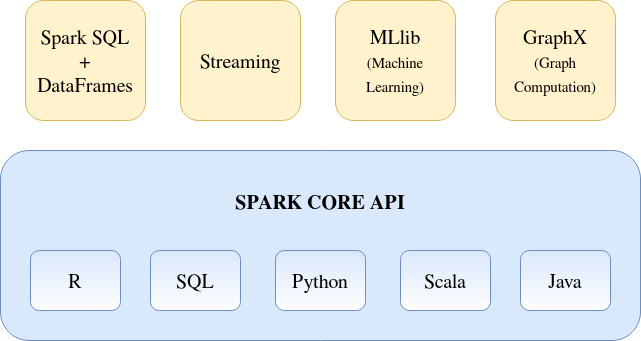
\includegraphics[width=250px]{Architecture/ApacheSpark.jpg}
    \caption{Apache Spark Modules}
\end{figure}
Here there is a brief description of each module:
\begin{itemize}
    \item \textbf{Spark Core}\\
    Spark Core is the base engine for large-scale parallel and distributed data processing. It is responsible for memory management and fault recovery, scheduling, distributing and monitoring jobs on a cluster and interacting with storage systems. Spark Core API is available in R, SQL, Python, Scala and Java.
    \item \textbf{Spark Streaming}\\
    Spark Streaming is the component of Spark which is used to process real-time streaming data. Thus, it is a useful addition to the core Spark API. It enables high-throughput and fault-tolerant stream processing of live data streams.
    \item \textbf{Spark SQL and DataFrames}\\
    Spark SQL is a module of Spark which integrates relational processing with Spark’s functional programming API. This module makes Spark ideal for extracting data from databases as well as for storing new data inside them.
    \item \textbf{GraphX}\\
    GraphX is the Spark API for graphs and graph-parallel computation.
    \item \textbf{MLlib (Machine Learning)}
    MLlib stands for Machine Learning Library. Spark MLlib is used to perform machine learning in Apache Spark. This module can be used in order to extract valuable knowledge from our data assets.
\end{itemize}
Given the fact that Apache Spark is an open-source framework (it is under the "Apache Licence 2.0", that is compliant with the Digital Public Good Standards), and given that it's modules implement all the functionality needed by our data-driven software, it is a reasonable choice to adopt Apache Spark framework in order to implement the big-data tier.

\section{Deployment View}
The following deployment diagram shows the system's physical layout, revealing which pieces of software run on what pieces of hardware:
\begin{figure}[H]
    \centering
    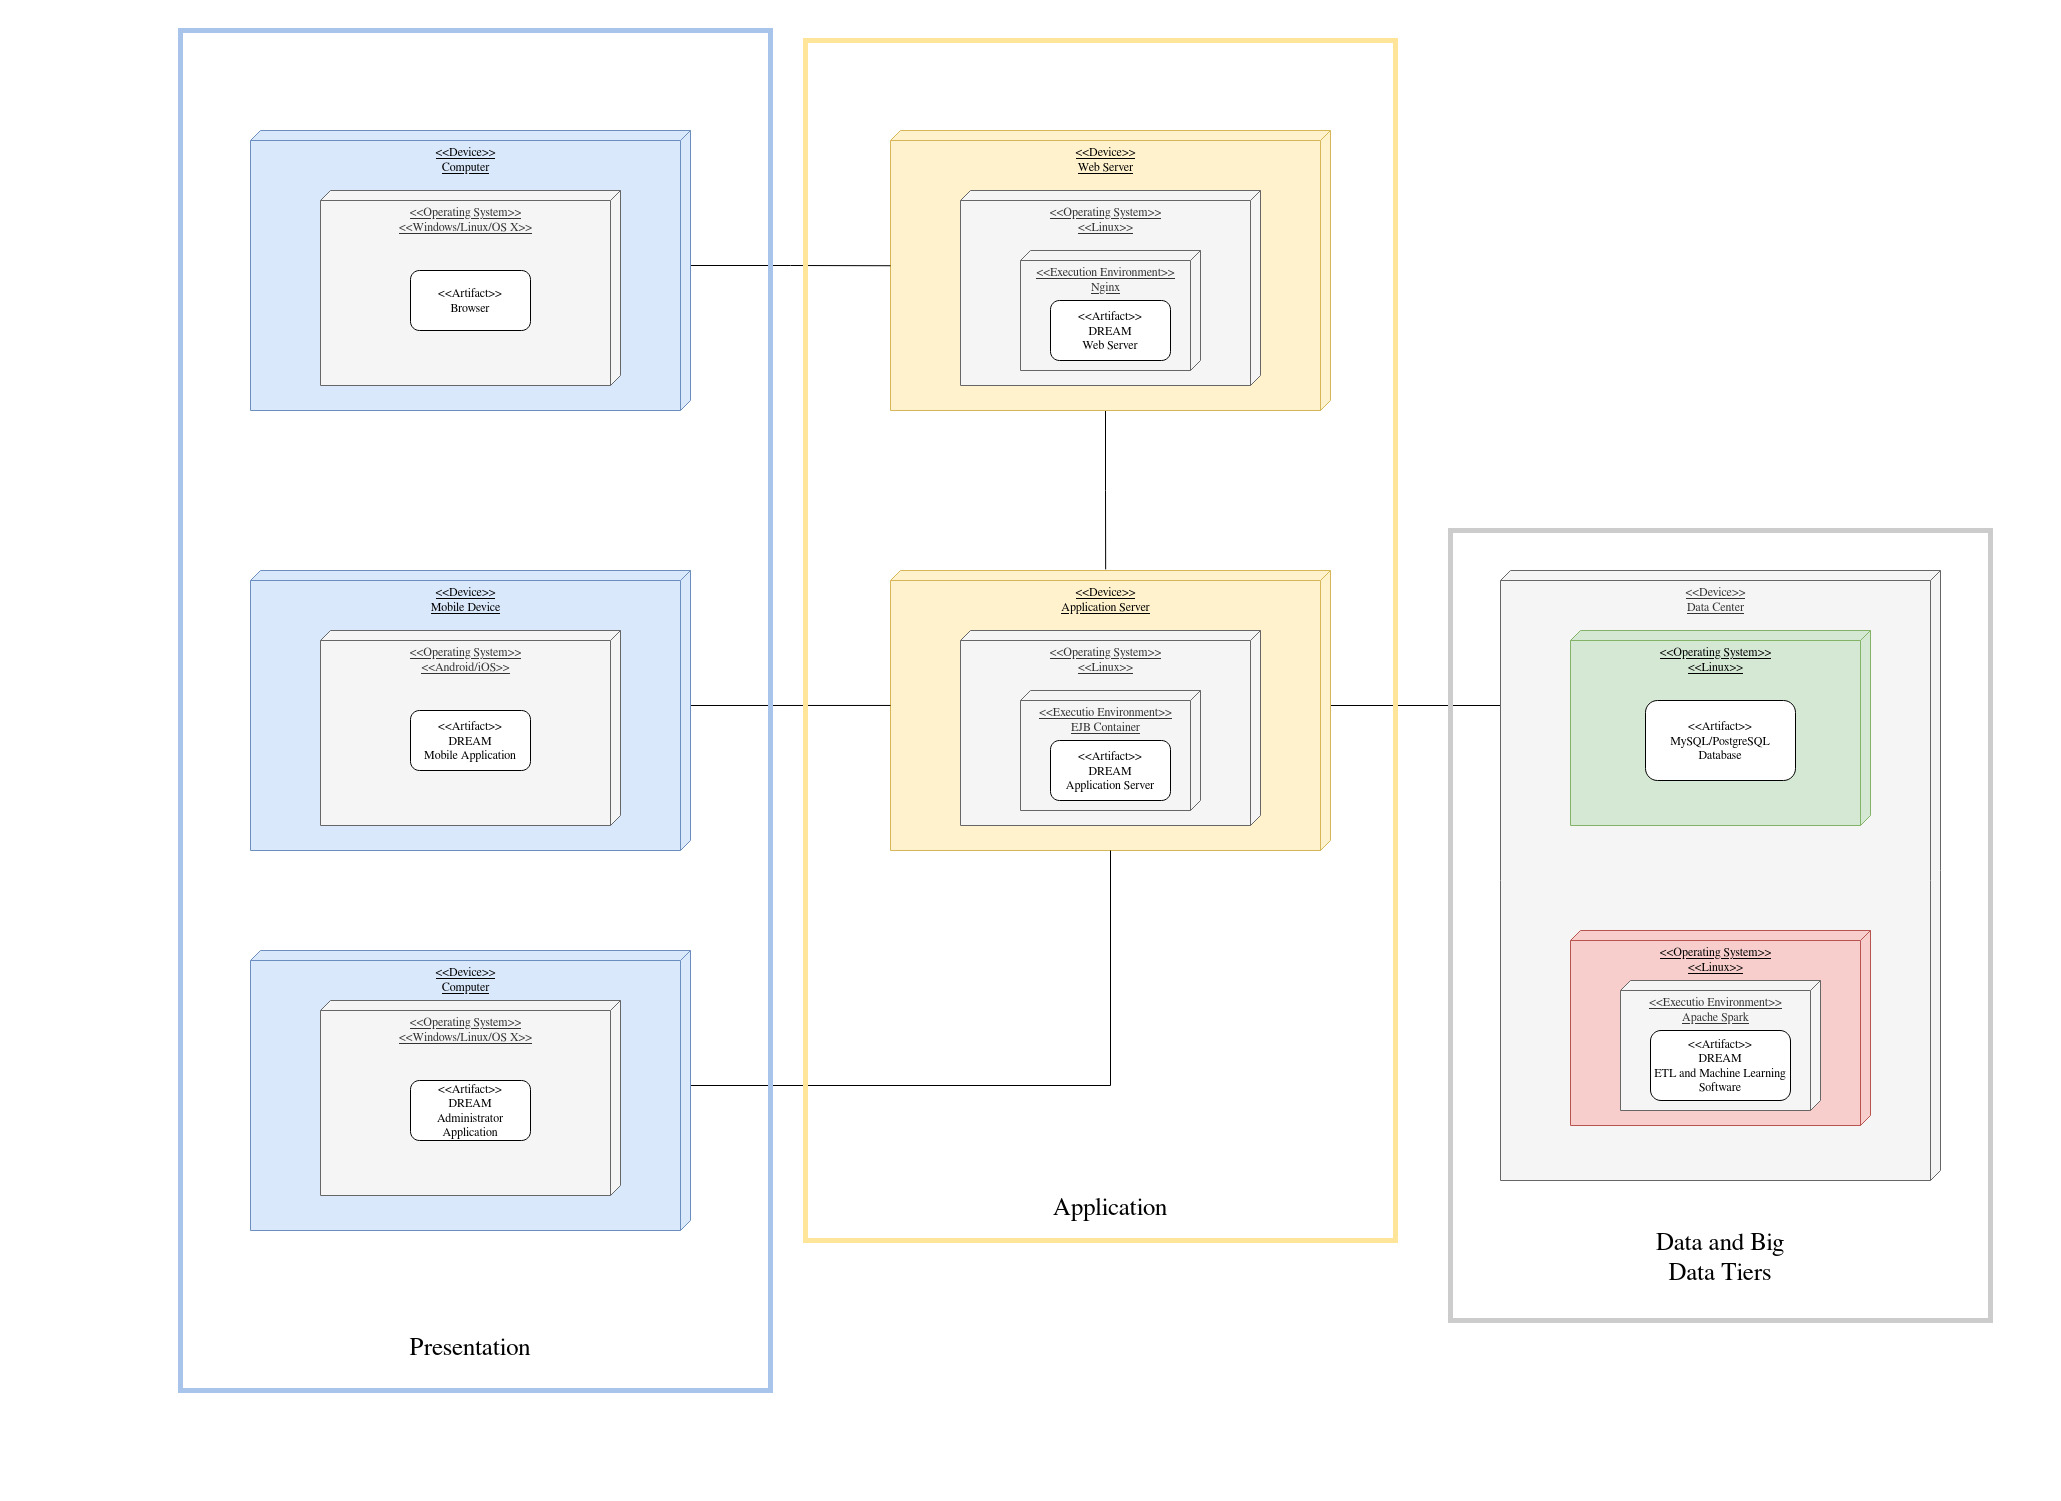
\includegraphics[width=400px]{Architecture/Deployment.jpg}
    \caption{Deployment Diagram}
\end{figure}
In the following will be given a brief description of each node:
\begin{itemize}
    \item \textbf{Computer}: Each user (farmers, agronomists and policy makers) can login into the system by using any type of personal computer through their favourite web browser. The browser will communicate with a web server.\\ System's administrators, instead, will be able to communicate directly with the application server by using a dedicated application.
    \item \textbf{Mobile device}: Each user farmers, agronomists and policy makers) will be able to download the official \emph{DREAM} application on their smartphone or tablet. The official application will communicate directly with the application server, thus acting like a thick client.
    \item \textbf{Web Server}: This node provide access to the application server's service to all the user that access the system through a web browser. In particular, the web server does not execute any business logic, but simply receive requests from the client, route them to the application servers and serve an HTML file to the client, which will build the page thanks to client-side scripting. This node can be replicated in order to handle large user traffic.
    \item \textbf{Application Server}: The application server contains the business logic of the entire system. Moreover, it communicates to the client tier through APIs, which will be used from the web servers (in case of web application) and the native application (in case of mobile app download). Furthermore, it communicates to the data tier through the DBMS gateway. This node can be replicated in order to handle large user traffic.
    \item \textbf{Data Center}: Because of the large amount of computation that the system must perform on data, the software concerning what we called "Big-Data tier" must be deployed on a data center. Similarly, in order to store a huge amount of data and to access them instantly, also the database should be deployed in the same data center where the ETL and Machine Learning software has been deployed.
\end{itemize}
\section{Runtime View}
The following sequence diagrams show how the components interact with each other whilst the functionalities
are executed.\\It has been assumed that the users interact with the application through web browser.\\
Nonetheless, the system operates in a very similar way from the mobile application. 
\\ Moreover, the interaction between the \textbf{Model} and the \textbf{DBMS} is omitted to enhance the readability of the diagrams. 


\subsection{Login}
\begin{figure}[H]
    \centering
    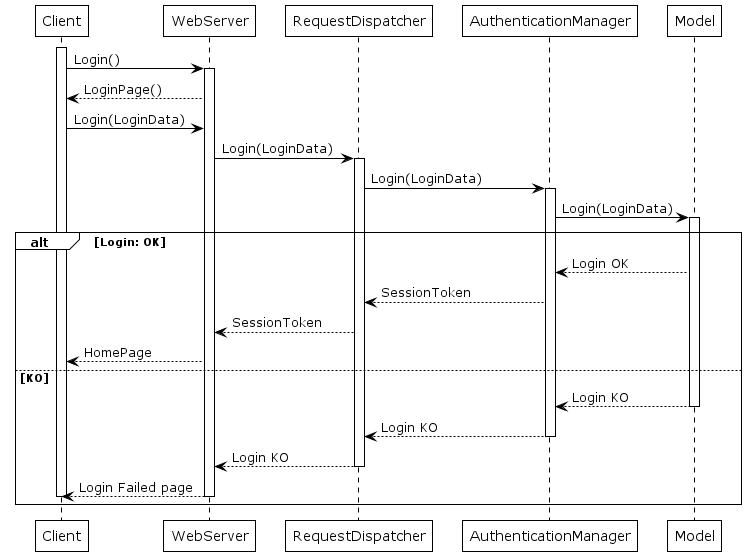
\includegraphics[width=400px]{SequenceDiagram/login.png}
    \caption{Runtime view: Login}
\end{figure}
This diagram represents the interactions that happen when a user of the software to be wants to login on the web application. \\The web application shows a login page with a login form. Once the login form is filled, the web application sends it to the \textbf{RequestDispatcher} that routes the request to the \textbf{AuthenticationManager}.\\ The AuthenticationManager knows how to contact the model component which interacts with the DBMS. \\If the login is successful a session token is set, otherwise the web application simply returns an error page. \\In all of the following sequence diagrams, the client is supposed to be correctly logged into the web application.

\subsection{Sign up}
\begin{figure}[H]
    \centering
    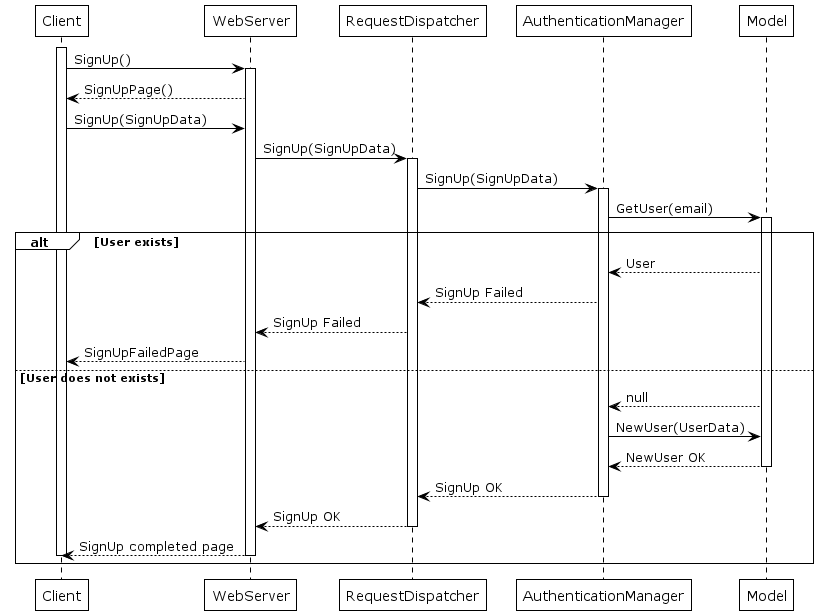
\includegraphics[width=400px]{SequenceDiagram/signup.png}
    \caption{Runtime view: Sign up}
\end{figure}
This diagram represents the interactions that happen when a user of the software to be wants to sign up on the web application.\\ The web application shows a sign up page with the appropriate form. Once the form is filled, the web application sends it to the \textbf{RequestDispatcher} that routes the request to the \textbf{AuthenticationManager}.\\
The AuthenticationManager knows how to contact the model component which interacts with the DBMS. 
In particular, the \textbf{AuthenticationManager} checks if the email provided by the client is already present in the system: if so the sign up request is rejected, the web application displays an error page.\\ Otherwise, the \textbf{AuthenticationManager} asks the Model to create a new user, and when the operation is completed, it tells the \textbf{RequestDispatcher} that the request was completed.\\ The web application then shows a page showing that the signup is completed.
\subsection{Farmer asks help through the chat}
\begin{figure}[H]
    \centering
    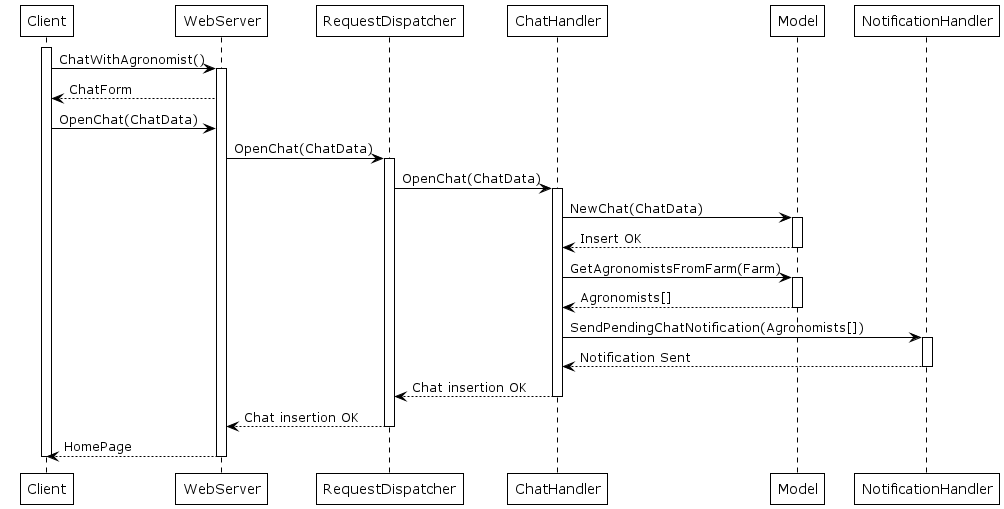
\includegraphics[width=400px]{SequenceDiagram/Farmer_1_2.png}
    \caption{Runtime view: Farmer asks help through the chat}
\end{figure}
This sequence diagram shows what happens when an already logged Farmer wants to open a chat.\\
The web application takes in input the request from the farmer and sends it to \textbf{RequestDispatcher}.\\ It knows that this request has to be processed by the \textbf{ChatHandler}, so the request routed to this component.
The \textbf{ChatHandler} has two tasks: it needs to insert the chat into the DBMS, and to notify the agronomists that belong to the same area of the farmer.\\ To complete the latter task, the \textbf{ChatHandler} must retrieve the agronomists that need to be notified about the new chat.\\ When those tasks are completed the \textbf{ChatHandler} returns to \textbf{RequestDispatcher} with a response telling that the operation was successful.\\
The \textbf{web application} then displays the home page again.


\subsection{Farmer creates a new thread in the forum}
\begin{figure}[H]
    \centering
    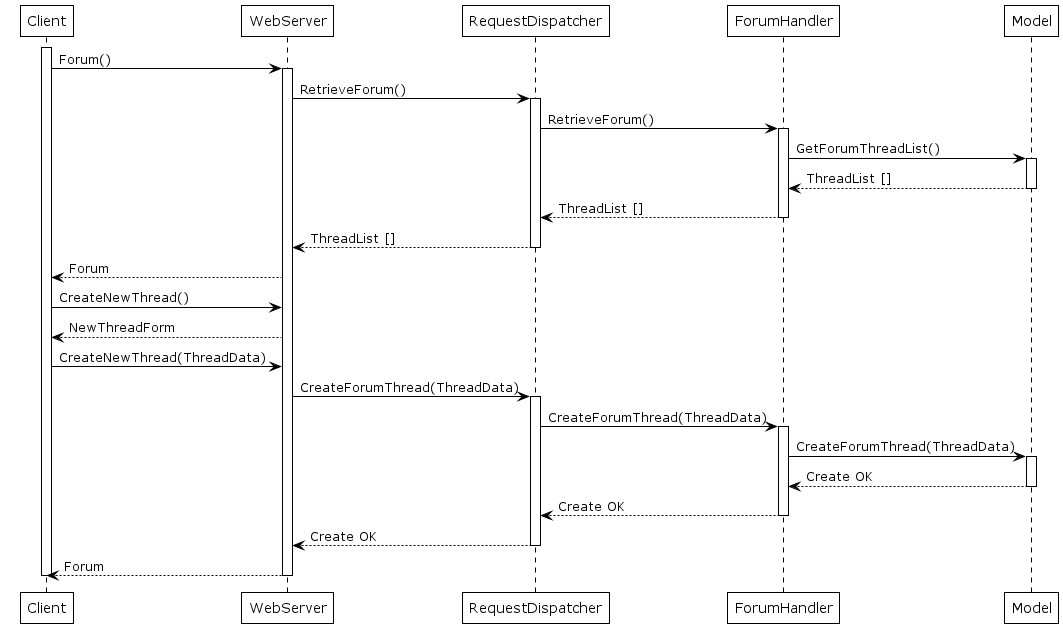
\includegraphics[width=400px]{SequenceDiagram/Farmer_1_7.png}
    \caption{Runtime view: Farmer creates a new thread in the forum}
\end{figure}
This sequence diagram shows what happens when an already logged \textbf{Farmer} wants to create a new thread in the forum.

When the Farmer wants to see the forum the web application needs to retrieve it from the DBMS. The request is routed from the \textbf{RequestDispatcher} to the \textbf{ForumHandler} that contacts the model to obtain what is needed to display the forum.\\ When the web application shows the forum the farmer selects the option to create a new thread.\\
So a form is displayed by the web application to the user, in order to collect the data about the new thread. The web application sends to the RequestDispatcher the request to create a new thread, with the associated data coming from the farmer input. \\The \textbf{ForumHandler} deals with this request by asking the model to create a new thread into the DBMS. If the insert on the DBMS is ok the \textbf{ForumHandler} returns to the \textbf{RequestDispatcher} that will return to the web application.\\ The farmer is then showed the updated forum page.


\subsection{Farmer inserts production data about their farm}
\begin{figure}[H]
    \centering
    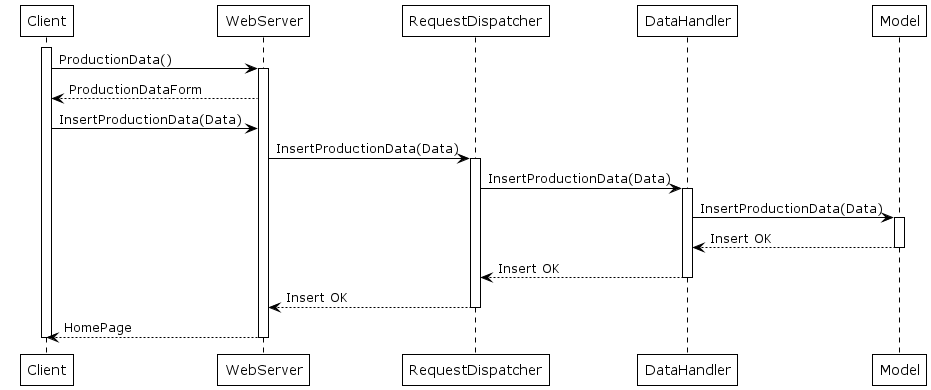
\includegraphics[width=400px]{SequenceDiagram/Farmer_1_9.png}
    \caption{Runtime view: Farmer inserts production data about their farm}
\end{figure}
This sequence diagram shows what happens when an already logged \textbf{Farmer} wants to insert production data about their farm.

When the form is filled by the farm, the web application sends to the \textbf{RequestDispatcher} a request to insert production data.\\ The request is routed from the \textbf{RequestDispatcher} to the \textbf{DataHandler}.\\ The request is processed and then the \textbf{DataHandler} interacts with the \textbf{Model} to persist the data. If the insert on the DBMS is ok the \textbf{DataHandler} returns to the \textbf{RequestDispatcher} that will return to the web application.\\ The farmer is then showed the home page.

\subsection{Agronomist takes charge of a chat request}
\begin{figure}[H]
    \centering
    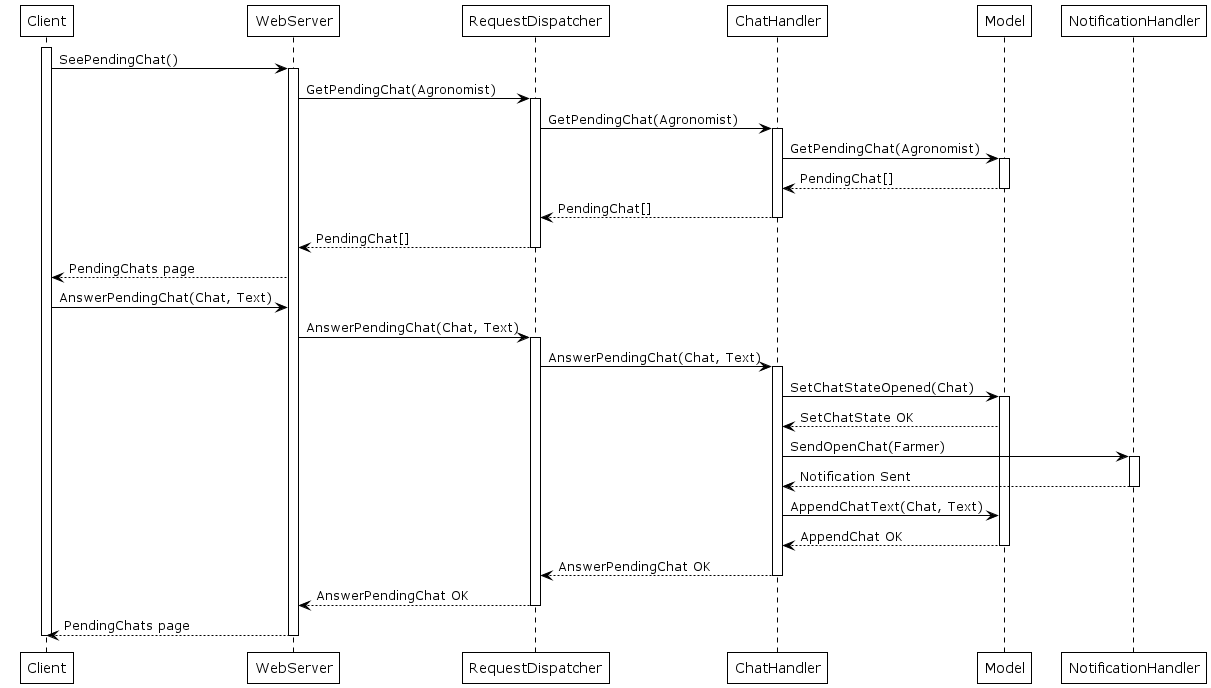
\includegraphics[width=400px]{SequenceDiagram/Agronomist_2_2.png}
    \caption{Agronomist takes charge of a chat request}
\end{figure}
This sequence diagram shows what happens when an already logged \textbf{Agronomist} wants to take charge of a chat request.

When the Agronomist asks to see the chat request in pending state, the \textbf{web application} asks the \textbf{RequestDispatcher} that routes the request to the \textbf{ChatHandler}.\\ It retrieves the pending chats associated to the area of the Agronomist. When the Agronomist answer the chat, the request that was routed again to the \textbf{ChatHandler} is processed. 
In fact, the \textbf{ChatHandler} updates the state of the chat (from pending to opened) and then asks the \textbf{NotificationHandler} to notify the Farmer that their chat has been opened. Then, if provided, the answer coming from the agronomist is appended to the chat. If the both the operation on the DBMS are successful, and the NotificationHandler confirms that the notification has been sent, the \textbf{ChatHandler} returns a positive answer to the \textbf{RequestDispatcher}.\\ The web application then shows the updated pending chats page.




\subsection{Agronomist schedules a visit to a farm}
\begin{figure}[H]
    \centering
    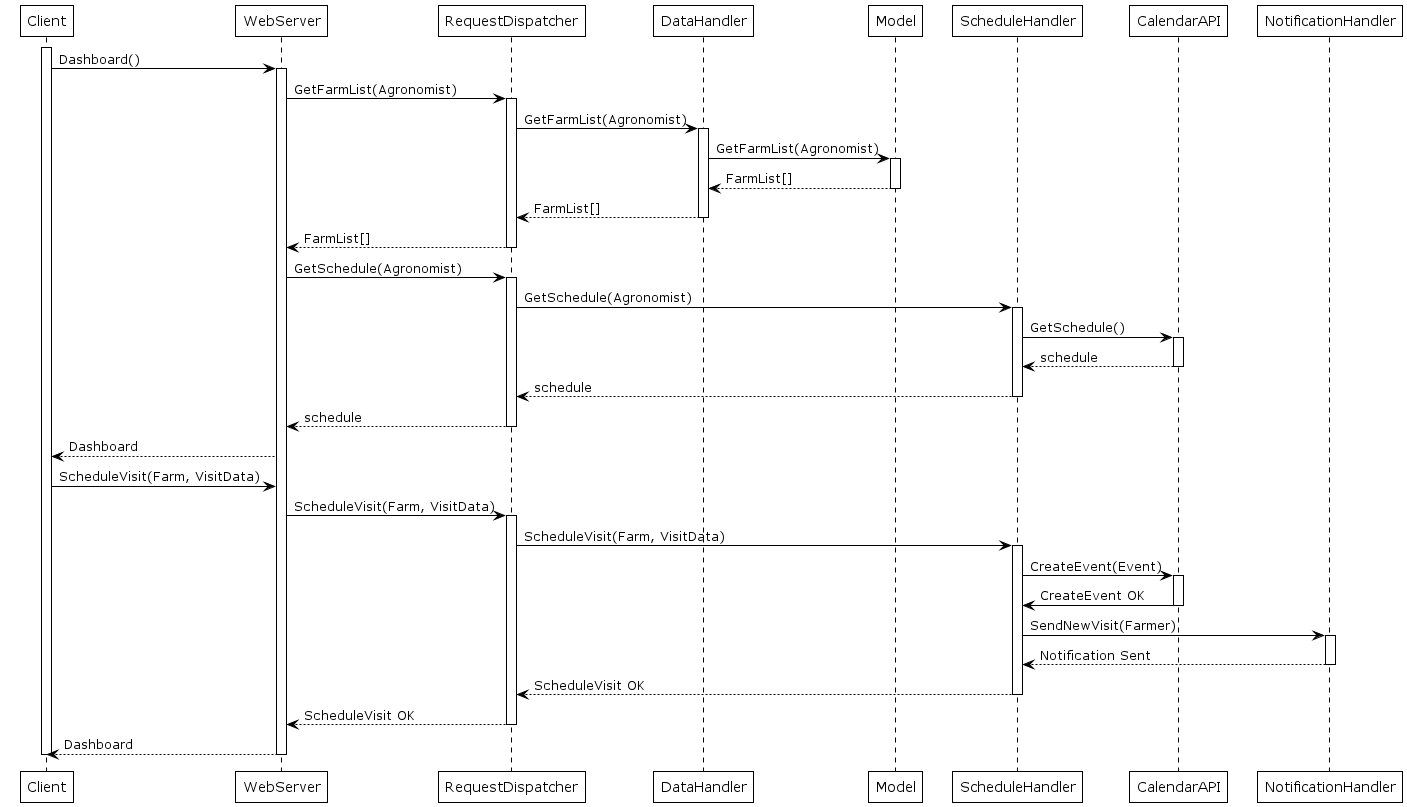
\includegraphics[width=400px]{SequenceDiagram/Agronomist_2_3.png}
    \caption{Agronomist schedules a visit to a farm}
\end{figure}
This sequence diagram shows what happens when an already logged \textbf{Agronomist} wants to schedule a visit to a farm.\\

The Agronomist want to see the dashboard. The web application retrieves it in two steps.\\ First, going through the RequestDispatcher, gets the farm list from the \textbf{DataHandler}.\\
Second, always going through the RequestDispatcher, gets the schedule from the \textbf{ScheduleHandler}. This component is the one that interacts with the external \textbf{Calendar API}. \\
Once the dashboard is displayed, the Agronomist can select a farm, and schedule a visit selecting time and date of the visit. \\
The request is routed to the \textbf{ScheduleHandler}: it creates the event in the calendar using the external \textbf{Calendar API} and then asks the \textbf{NotificationHandler} to notify the farmer that a visit to their farm has been scheduled.



\subsection{Agronomist confirms a scheduled visit}
\begin{figure}[H]
    \centering
    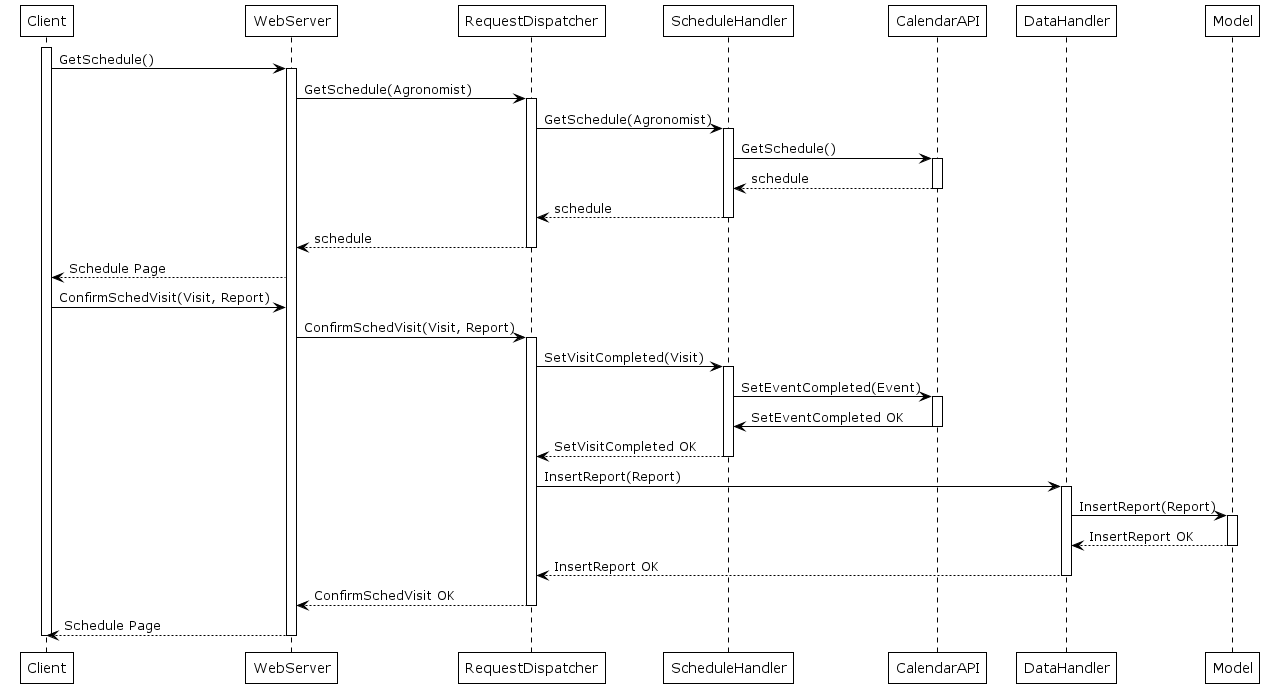
\includegraphics[width=400px]{SequenceDiagram/Agronomist_2_4.png}
    \caption{Agronomist confirms a scheduled visit}
\end{figure}
This sequence diagram shows what happens when an already logged \textbf{Agronomist} wants to confirm a scheduled visit.\\
As already clarified in RASD document, this action allows the Agronomist to confirm that he actually visited a farm, that was planned in their schedule. This means also that a report must be provided.\\

The web application retrieves the schedule, from the \textbf{ScheduleHandler} that interacts with the external \textbf{Calendar API}.\\
Then the Agronomist can select a past visit, and requests to confirm it. Here the Agronomist must insert the report of the visit. \\
The request, is sent to the \textbf{RequestDispatcher}. Here the dispatcher has to interacts with two side of the application logic, the one associated to the scheduling of the visits (the \textbf{ScheduleHandler}), and the one associated with the data (the \textbf{DataHandler}).\\
First, it contacts the \textbf{ScheduleHandler} to change the state of the visit to "completed".\\
Then it has to store persist the report associated with the visit in the internal DBMS, through the \textbf{DataHandler}.




\subsection{Agronomist cancels a scheduled visit}
\begin{figure}[H]
    \centering
    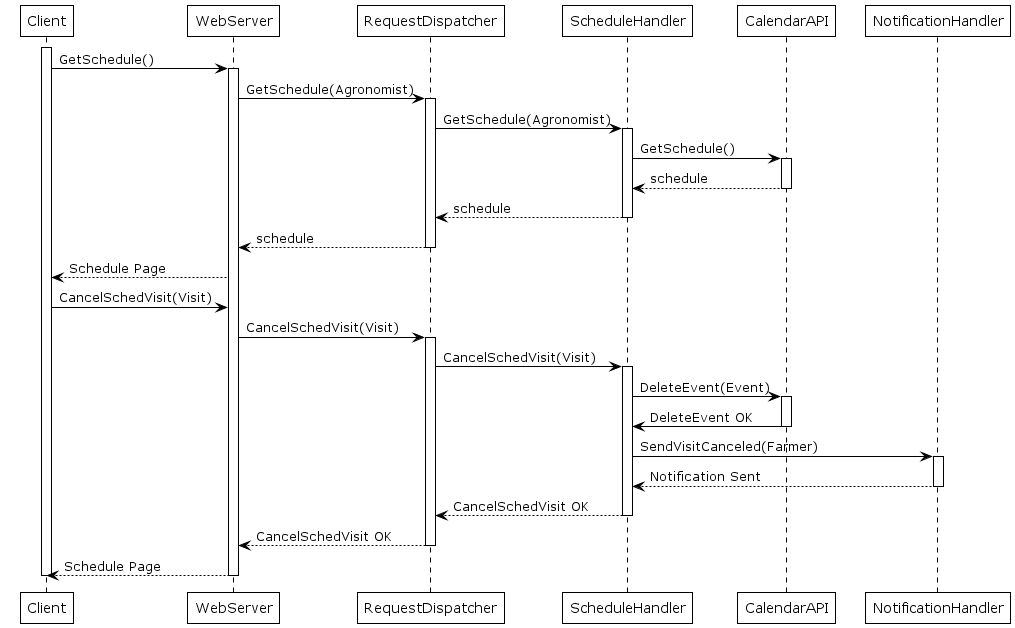
\includegraphics[width=400px]{SequenceDiagram/Agronomist_2_5.png}
    \caption{Agronomist cancels a scheduled visit}
\end{figure}
This sequence diagram shows what happens when an already logged \textbf{Agronomist} wants to cancel a scheduled visit.\\

Right after the retrieving of the schedule, the Agronomist selects a visit to cancel it.
The request goes to the \textbf{ScheduleHandler} that interacts with the external \textbf{Calendar API} to delete the event. \\ 
Furthermore, the \textbf{ScheduleHandler} knows that, dealing with a request to cancel a visit, it has to tell the farmer that the visit is canceled. This is why it contacts the \textbf{NotificationHandler}, that returns when the notification is sent. \\
At this point, the \textbf{ScheduleHandler} can confirm to the web application (through the RequestDispatcher) that the operation went well.
\section{Component Interfaces}
The following diagram shows the methods mentioned in the sequence diagrams of the previous section. Furthermore, it clarifies to which interface belongs each method and how the components and interfaces interact with each other in the system.
The names of the methods defined in the
interfaces are self-explanatory and are not meant to be followed precisely by the
developers. They are just a simplified representation of what the different
components can offer and how they interact with each other. This artifact should clarify  how the system structure is organized to the stakeholders as well as being a simple guideline for the developers.


\begin{figure}[H]
    \centering
    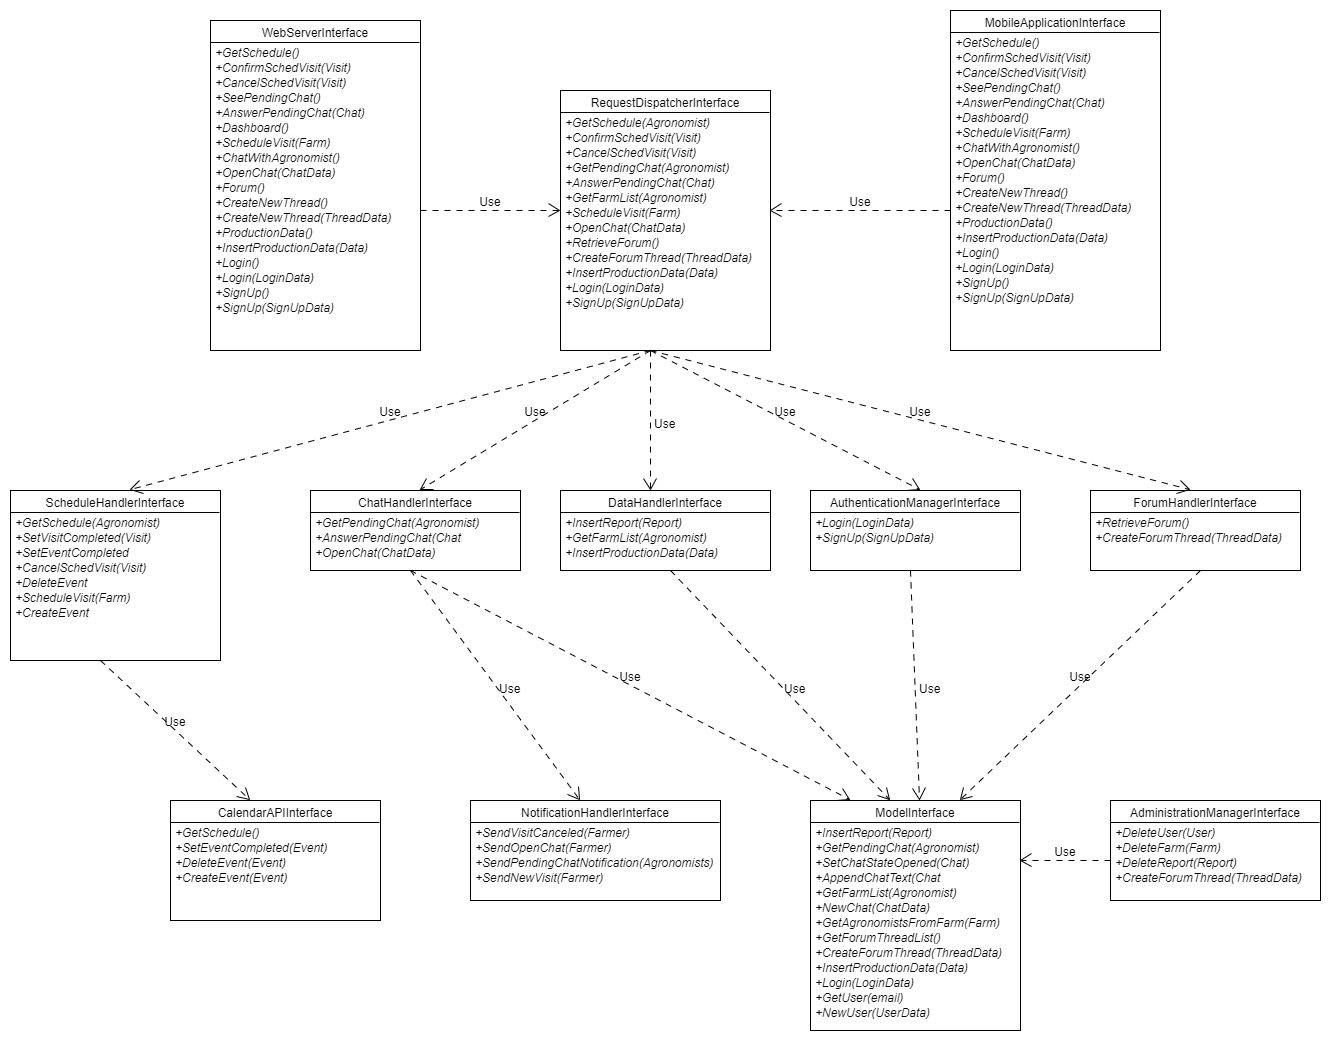
\includegraphics[width=400px]{Interface/int_diagram2.png}
    \caption{Component Interface}
\end{figure}

\section{Selected Architectural Styles and Patterns}
\subsection{Four-Tiered Architecture}
The first three tier of the architecture designed by us are the well known three tiers of a standard three tier architecture:
\begin{itemize}
    \item Presentation tier
    \item Application tier
    \item Data tier
\end{itemize}
This division has numerous advantages in terms of:
\begin{itemize}
    \item \emph{Maintainability}: each tier can be updated and replaced independently without affecting the others
    \item \emph{Scalability}: each tier can be scaled independently of the others as needed
    \item \emph{Load distribution}:each tier can be replicated if needed without affecting the functioning of the other tiers, thus allowing the system to distribute the load of the system on more machines easily
\end{itemize}
The fourth tier was adopted by us in order to handle the ingestion, processing, and analysis of data that is too large or complex for traditional database systems.
\subsection{RESTful Architecture}
The RESTful application is adopted both on web and mobile side.
Because of the principles explained before, the REST architectural style provides:
\begin{itemize}
    \item Scalability of components interaction
    \item Generality of interfaces
    \item Independent deployment of components
    \item Intermediary components to reduce latency, enforce security and encapsulate legacy systems
\end{itemize}
\subsection{Model View Controller (MVC) Pattern}
The model view controller pattern will separate components in three layers:
\begin{itemize}
    \item Model: it manages the data and that communicates with the controller
    \item View: it is in charge of the visualizations
    \item Controller: it controls the ways in which the interfaces react to the user input and interacts with the data model
\end{itemize}
The MVC pattern helps to break up the front-end and back-end code into separate components. This way, it's much easier to manage and make changes to either side without them interfering with each other.\\ \\
Moreover, this pattern applies perfectly to the architecture chosen, in fact there is a mapping between presentation tier and view components, application tier and controllers, data tier and model.
\chapter{User Interface Design}
Here is an overview on how the system will look like.\\ \\
\textit{Notice that there are no mockups for the \textbf{IT adiminstrator} because those are very similar to the one that we present here, except for the fact that, of course, the IT adiminstrator will have more control over all the buttons and will have the possibility to manage all the parts of the system while the other actors have a more restricted scope.}
\section{Login and sign-up screens}
This view has the goal of showing how the three different Actors are managed a registration phase and, of course, at login phase, as well.
Notice that registration screen is divided in two parts, but while the first part is mandatory for all the three actors, the second part is mandatory only for \textbf{Farmers} and \textbf{Agronomists}.    \\
The \textbf{Policy Maker} would end the registration at the second step, just entering some personal information, while the \textbf{Agronomist} must insert a list of areas in which they can operate, knowing that the division about the areas has already been shown to them. For what concerns the Farmer, they must insert their farm location.

\begin{figure}[H]
    \centering
    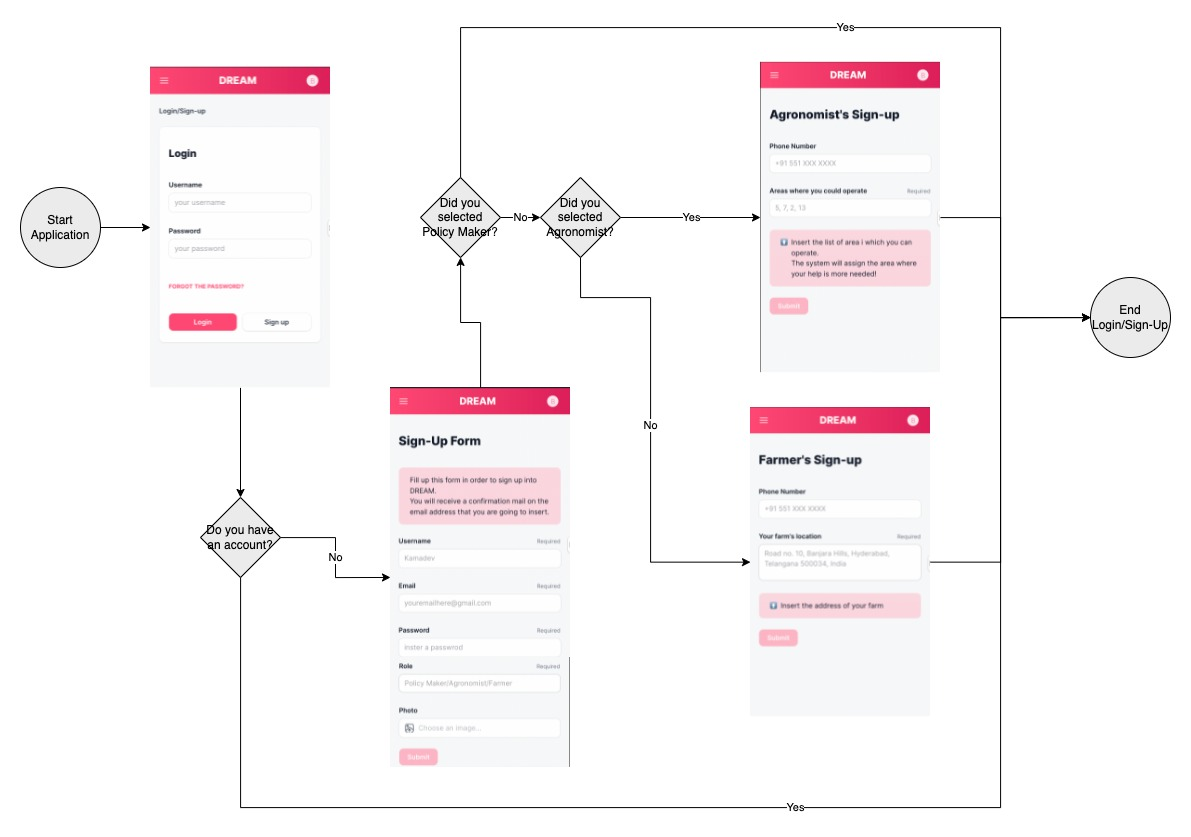
\includegraphics[width=400px]{Mockups/MockUpDiagram-login_signup.jpg}
    \caption{Login and sign-up screens}
\end{figure}

\section{Farmer's navigation}
We want to present also, at \textit{Figure 3.2}, the classical possible navigation of a \textbf{Farmer}. From the homescreen which present 5 buttons, the first three useful for reaching the \textit{Form}, the open \textit{chats} and the \textit{farm}'s details, while the last 2 buttons are used in order to \textbf{ask for help}, from there it's possible to \textit{ask for a visit} to an Agronomist, and the second one is useful to open a \textit{chat request}. 
\subsection{Your Farm}
Tapping on the "Your Farm" button it's possible to reach the screen where some personal information are shown and are editable and, more important, information about the farm are displayed. The \textbf{Farmer} will be able to filter and group data about their farm by clicking on the appropriate buttons: \textit{see other data} and \textit{order by}.
\subsection{Forum}
Tapping on the "Forum" button it's possible to reach the Forum screen. This screen is reachable not only by the \textbf{Farmers} but also by all the \textbf{other actors}, we decided to show this screen in this navigation for seek on simplicity, the other actors will find the button to reach the forum in the \textit{Navigation menu} (the so called "hamburger menu"). 
In this screen are presented the threads that have been published, ordered as the user desire. Each item of this list shows the \textit{thread title}, the \textit{publication date} and the \textit{person who opened the thread}, with their respective role.\\
By tapping on a topic it's the text is shown, the screen allows to comment the topic or just have a look to the comments that already exists. 

\begin{figure}[H]
    \centering
    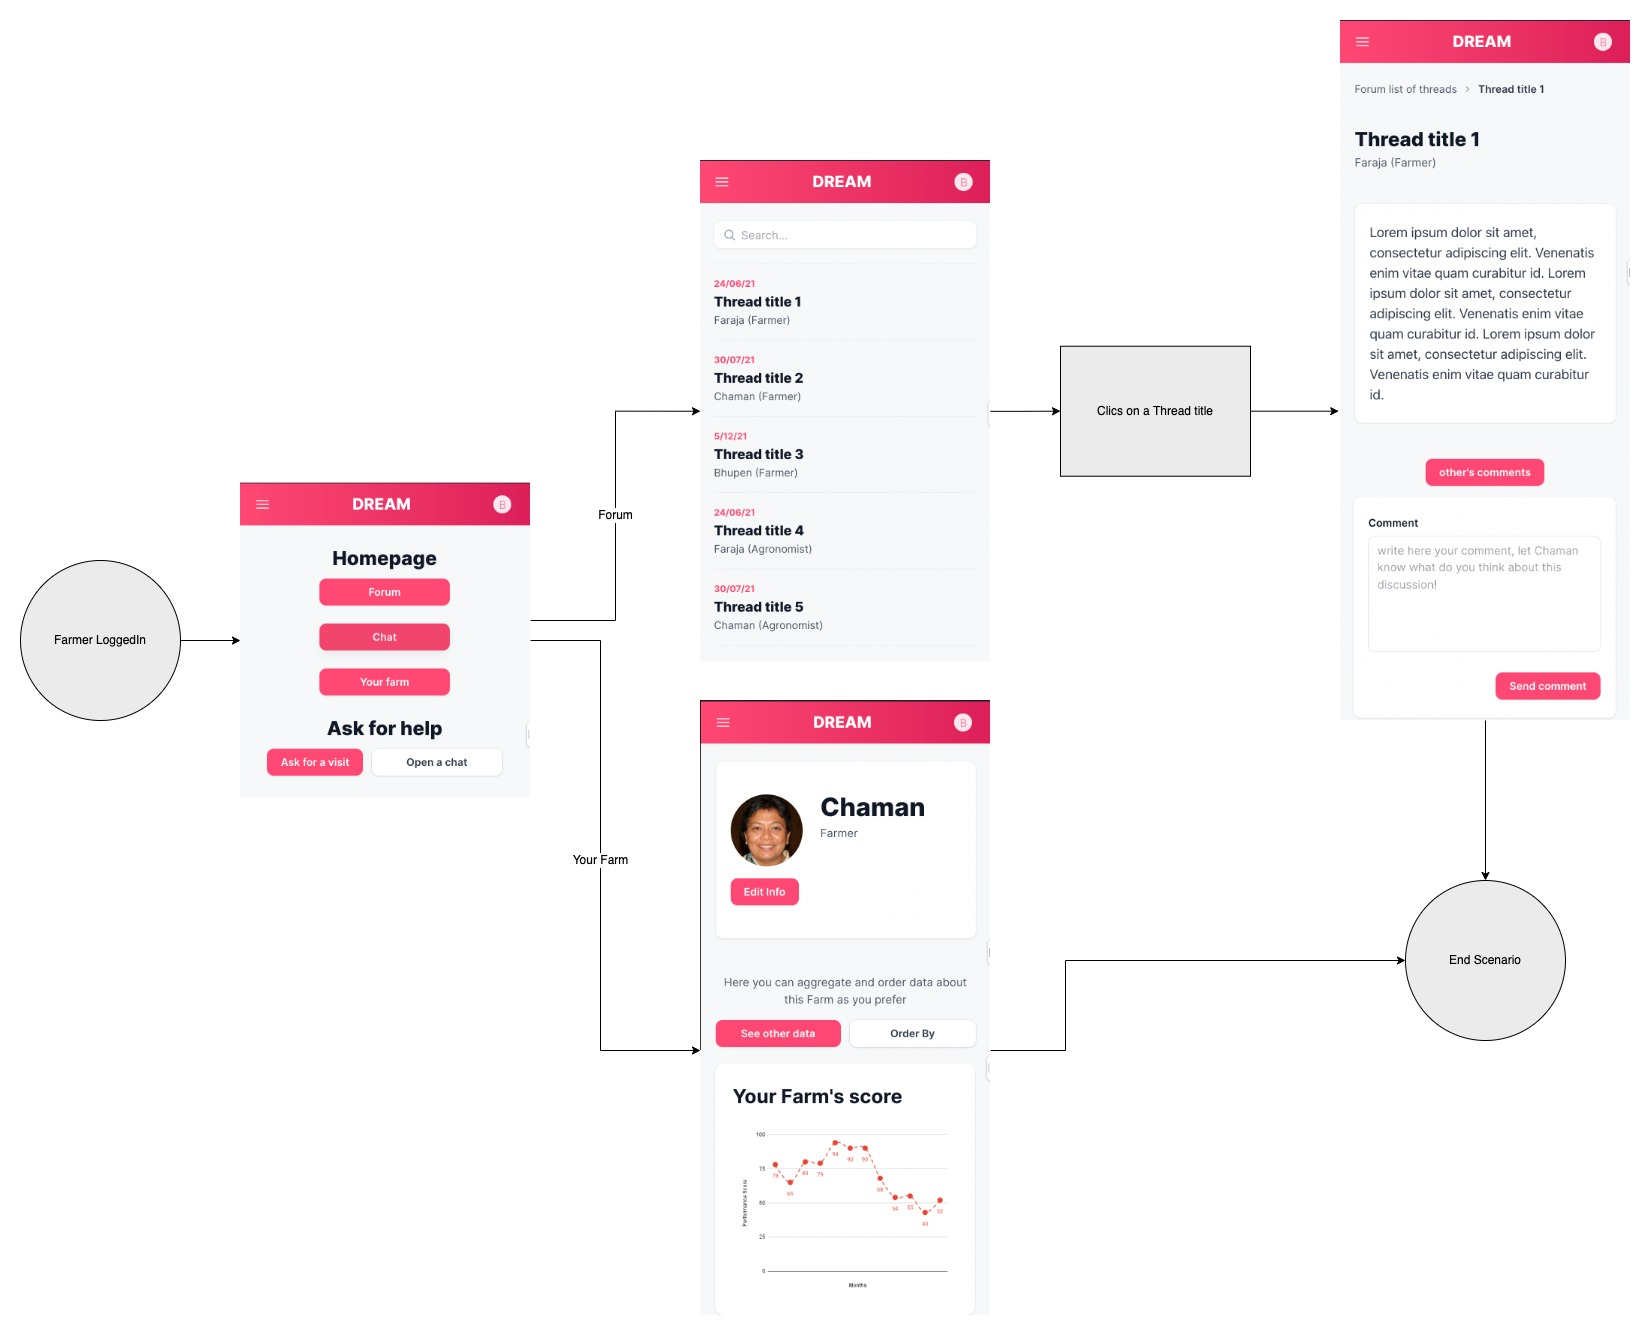
\includegraphics[width=400px]{Mockups/MockUpDiagram-Farmer.jpg}
    \caption{Farmer's main navigation}
\end{figure}

\section{Agronomist's navigation}
The \textbf{agronomist}, once logged, will see the list of the farms assigned to their area. The list is ordered by descendent priority. For each farm presented is possible to look for more details by tapping the button "Go!". \\
Once the Agronomist tapped on a farm all the details related with that farm are displayed. The agronomist will be able to look a different type of data using the proper buttons and will be also able to \textit{book a visit} or \textit{open a chat} with the farmer.

\begin{figure}[H]
    \centering
    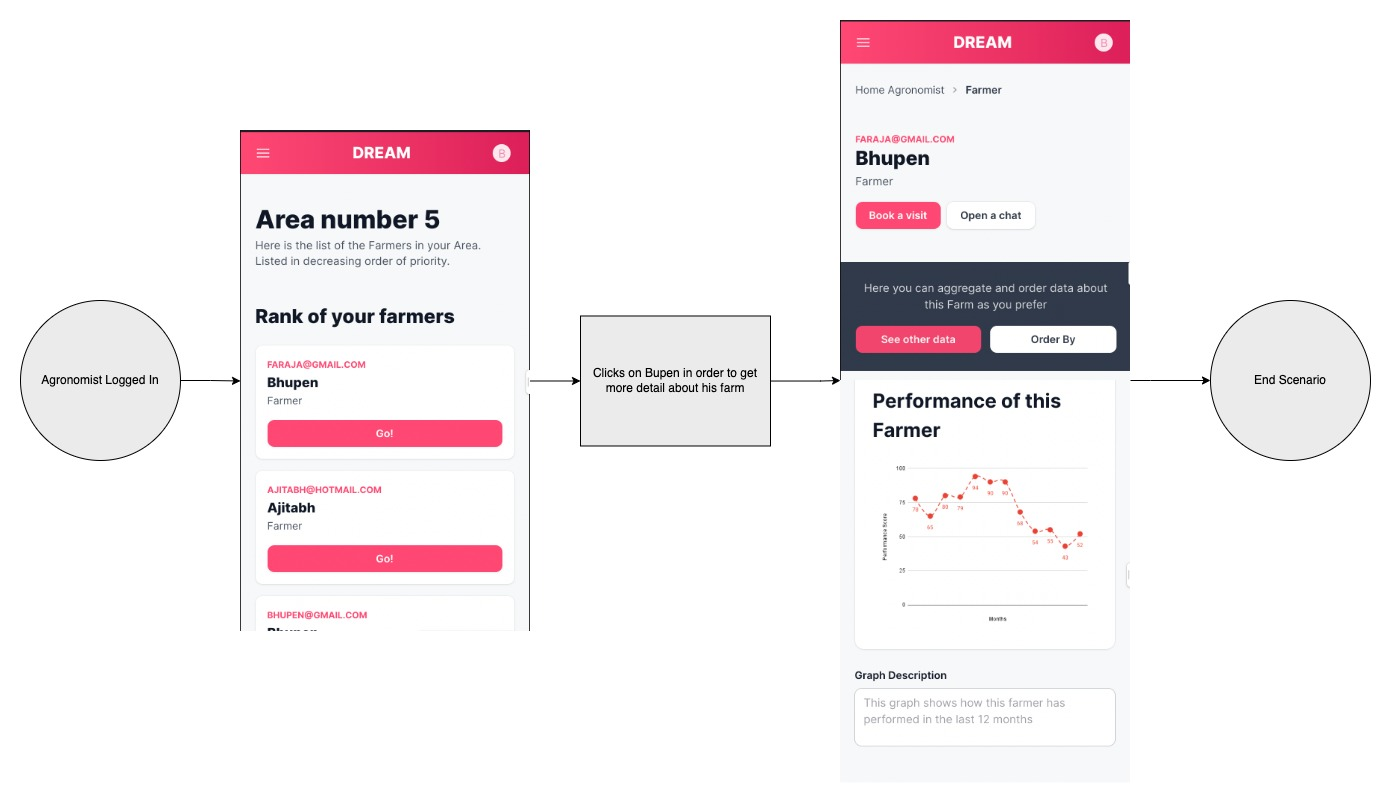
\includegraphics[width=400px]{Mockups/MockUpDiagram-DetailFarmAgronomist.jpg}
    \caption{Agronomist's main navigation}
\end{figure}

\section{Agronomist's schedule}
The \textbf{agronomist} will be able to came to this screed by using the navigation menu (the so called "hamburger menu"). Here is presented the schedule that the agronomist has previously prepared by \textit{booking appointments with some farmers}. It's possible to see, for each slot, the farmer that the agronomist has the appointment with, the hour the appointment is scheduled for and the farm's address.
Once an appointment is \textit{confirmed} by clicking the button "confirm". The \textit{report screen} is displayed, here the agronomist can insert all the measures that they have taken during the visit and write the detailed report about the status of the farm in order to simplify the tracking of the good policy. 

\begin{figure}[H]
    \centering
    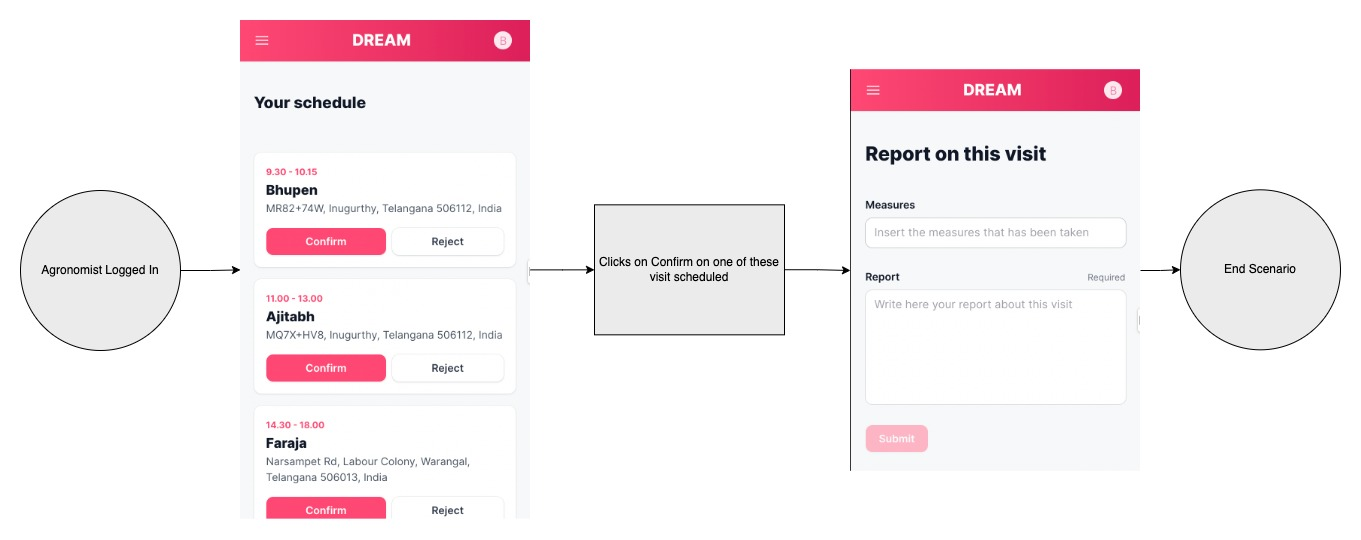
\includegraphics[width=400px]{Mockups/MockUpDiagram-ScheduleAgronomist.jpg}
    \caption{Agronomist's schedule view}
\end{figure}

\subsection{Chat request}
This screen is reachable by the agronomist through the navigation menu. Here is the list of the farmers that have sent a request to chat and are waiting for being taken into account by an agronomist of their area.
\begin{figure}[H]
    \centering
    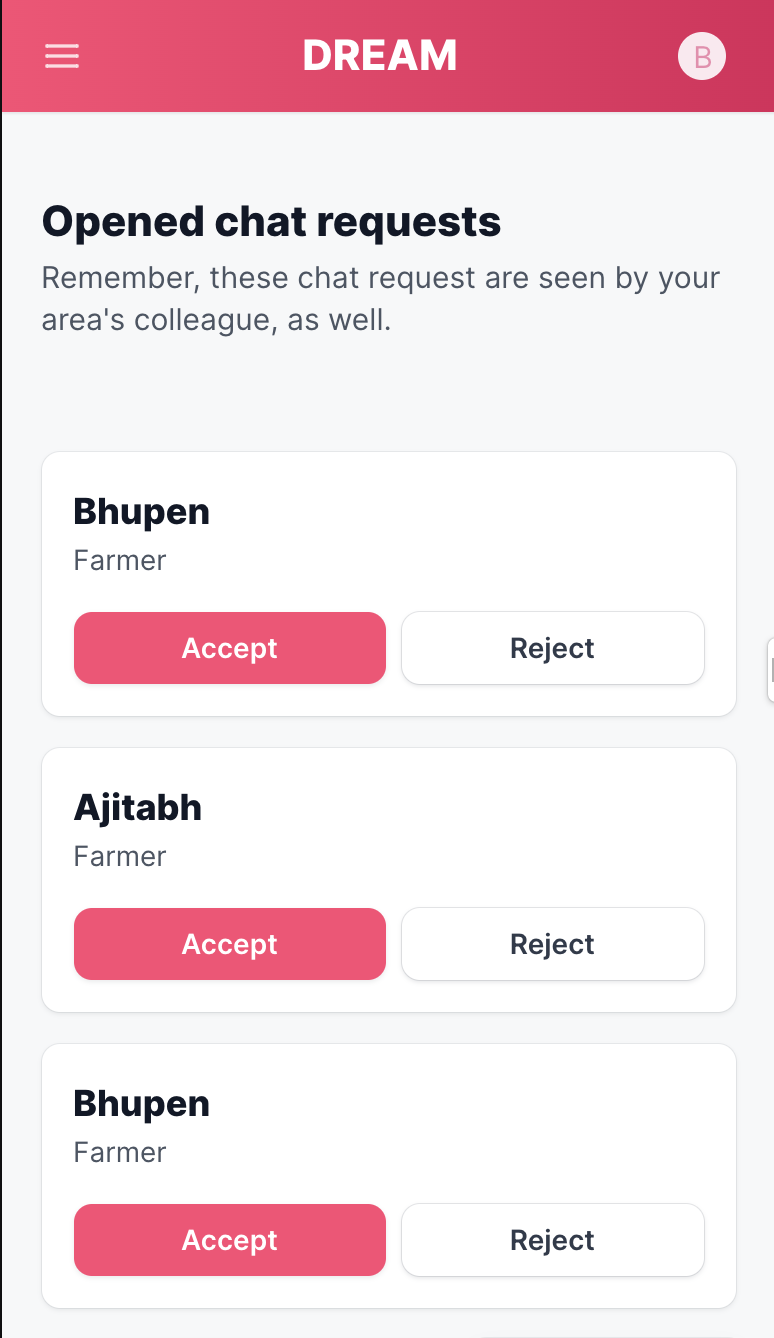
\includegraphics[width=150px]{Mockups/chatRequestAG.png}
    \caption{Chat request list, Agronomist's View}
\end{figure}

\subsection{Agronomist's profile}
Here is shown the agronomist profile. Which shows the data about how their area are performing. 
\begin{figure}[H]
    \centering
    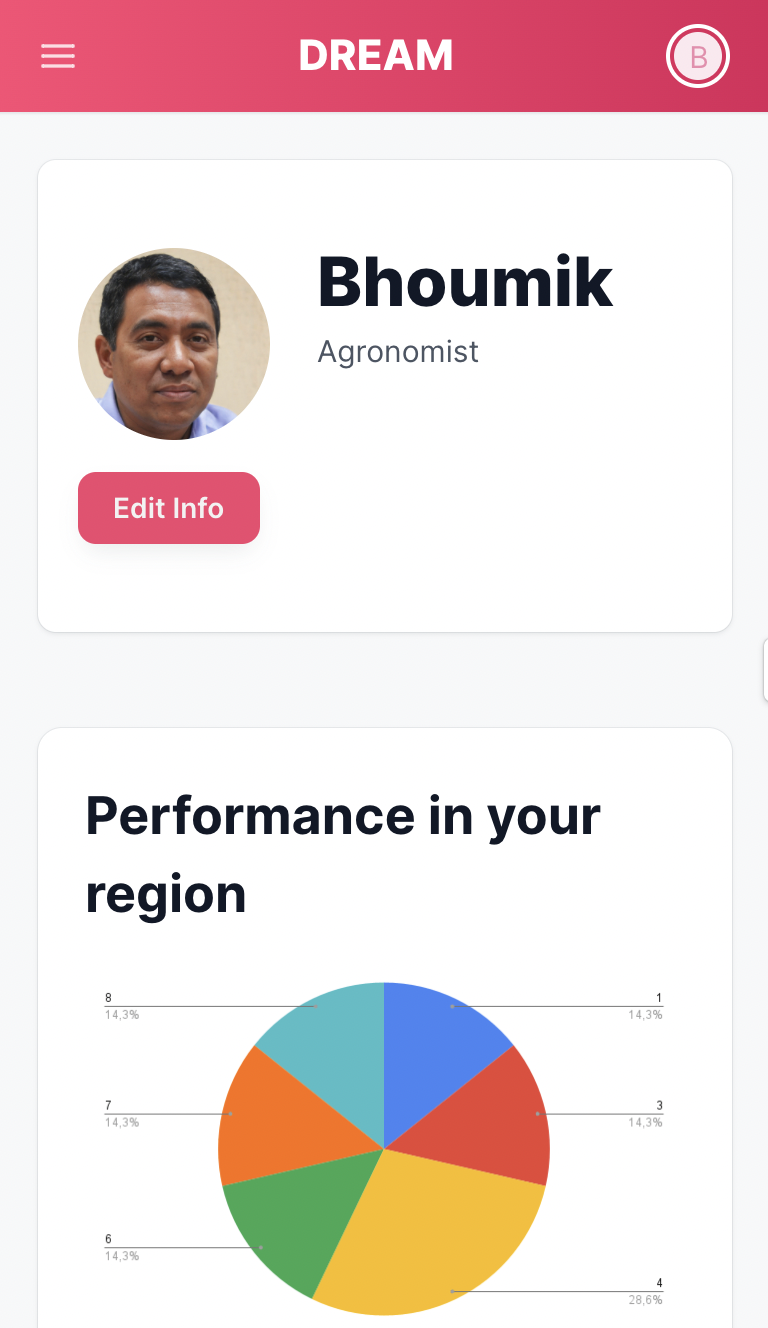
\includegraphics[width=150px]{Mockups/personalProfileAG.png}
    \caption{Agronomist's personal profile}
\end{figure}

\section{Note about the Policy Maker}
Here we didn't present a proper navigation for the policy maker because we assume that he has a lot more control over the others actors, so the most of the screens that has been presented here will be valid also for the \textbf{Policy Maker}. \\
For what concerns the "performance evaluation" we have just to say that they will have a proper button in the navigation menu that will allow them to reach a screen which will look like the agronomist's left one presented in the figure 3.3. The difference with respect to the agronomist's one is the scope of the list, the policy maker will, of course, see a list build among all the farmers in Telangana. And the detailed screen of each farmer will also give to the Policy Maker the possibility to download all the report written by any agronomist to that farm.\\ \\

If the user is navigating the system by using a web browser, their interface will look like the one in the following link: https://hungermap.wfp.org/.

\chapter{Requirements Traceability}
The entire design must ensure that the system can enforce all the requirements defined in the previous document (RASD) and consequently that the system can achieve the goals that have been established. This section will shown the traceability between requirements and modules described in component diagram.\\ \\
In order to make this document independent from the requirements and analysis document, all the requirements and the goals will be listed below:\\ \\
\textbf{Goals}
\begin{enumerate} [label=(G\arabic*), font=\itshape]
    \item \emph{Data-Driven approach}\\DREAM will be able to fetch data from different databases. Then, DREAM will be able to collect, analyze and perform inference on this data in order to extract new knowledge that will be at the service of different DREAM’s users.
    \item \emph{Help policy makers to implement better policies which will make Telangana’s agriculture better}\\DREAM will allow policy makers to see real time data regarding Telangana and Telangana’s farms. In particular they will be able to see which farms are performing well and which farms are performing poorly. Moreover, they will be able to understand which steering initiatives are working and which not.
    \item \emph{Help farmers to become weather resilient and increase their production} \\DREAM will allow farmers to see statistics regarding their farms. Moreover, DREAM will provide to them personalized suggestions based on the data regarding their farm and on the data regarding farms that are doing particularly well in similar environments.
    \item \emph{Facilitate and make systematic the communication between farmers and agronomists} \\DREAM will make communications between agronomists and farmers easy and stable. In fact, DREAM will allow farmers to chat with agronomists in just a few clicks. Moreover they will be able to request agronomists to visit them when they are facing complex problems. \\Agronomists, instead, will be able to access real time data regarding farms they are responsible for, and therefore they will be able to see which farms are performing well and which farms are performing poorly. Based on this knowledge, agronomists will be able to decide how much and when to visit each farm, and to send periodical reports to policy makers regarding how the farms (they are responsible for) are doing.
    \item \emph{Create a network of farmers} \\Through DREAM, farmers will be able to communicate between each other in order to exchange best practices and advice.
\end{enumerate}

\textbf{Requirements}
\begin{enumerate} [label=(R\arabic*), font=\itshape]
    \item The system allows users to sign up
    \item Every user can access the system only if they are registered
    \item The system must allow to access the system only if the credentials used are correct
    \item The system must not allow to register two different users with the same username
    \item The system must not allow the same user to register themselves more than once
    \item The system shall associate to each area one or more agronomists
    \item The system shall associate each farmer to one and only one area
    \item Each agronomist is associated to one and only one area
    \item The system allows the agronomist to see only the list of farms for which they are responsible of
    \item The system allows the farmer to see data about their farm
    \item The system must not allow the farmer to see data about farms other than theirs
    \item The system allows the agronomist to see data about a specific farm
    \item The system allows the agronomist to see data about the area for which they are responsible for
    \item The system must not allow the agronomist to see data about farms for which they are not responsible for 
    \item The system must not allow the agronomist to see data about an area for which they are not responsible for
    \item The system allows the policy maker to see data about a specific farm
    \item The system allows the policy maker to see data about an area
    \item The system allows the policy maker to see data about all the areas in Telangana
    \item The system must fetch data from different sources containing relevant information for the scope of the application
    \item The system must elaborate and aggregate data fetched from different sources
    \item The system allows farmers to request to have a chat with an agronomist
    \item The system allows agronomists to accept chat requests
    \item The system allows farmers and agronomists to interact through a chat
    \item A farmer, belonging to an area, can chat only with an agronomist belonging to the same area
    \item Each farmer can have at most one open chat at any given time
    \item Each agronomist can have multiple chats open at any given time
    \item The system allows only agronomists to close chats
    \item The system allows farmers to request a visit from an agronomist
    \item The system must show an agronomist a list of farms they have to visit, ordering them by priority
    \item The system must prioritize the farms that need help
    \item The agronomist must prioritize the farms that the system prioritize
    \item The system allows agronomists to schedule a visit at any farm of their competence
    \item The system allows agronomist to set up a daily schedule
    \item The system must notify a farmer when an agronomist schedules a visit to their farm
    \item The system must notify an agronomist when a farmers cancels a scheduled visit to their farm
    \item The system must notify a farmer when an agronomist cancels a scheduled visit to their farm
    \item The system allows agronomists to cancel a scheduled visits within one day before
    \item The system shall allow farmers to interact through a forum with other farmers and agronomists
    \item The system shall allow agronomists to interact through a forum with other agronomists and farmers
    \item The forum allow to each farmer or agronomist with each other no matter the area they belong to 
    \item The system shall allow agronomists to confirm what they have done during the day
    \item The system shall allow agronomists to insert a report regarding the visits they have done during the day
    \item The system shall allow to remove a visit from the agronomist’s screen only if they fill out the report
    \item The system shall allow agronomists to insert data regarding measurements taken during the visits done during the day
\end{enumerate}

The following table allows to see the mapping between the goals, the requirements and the components of the system:
\begin{figure}[H]
    \centering
    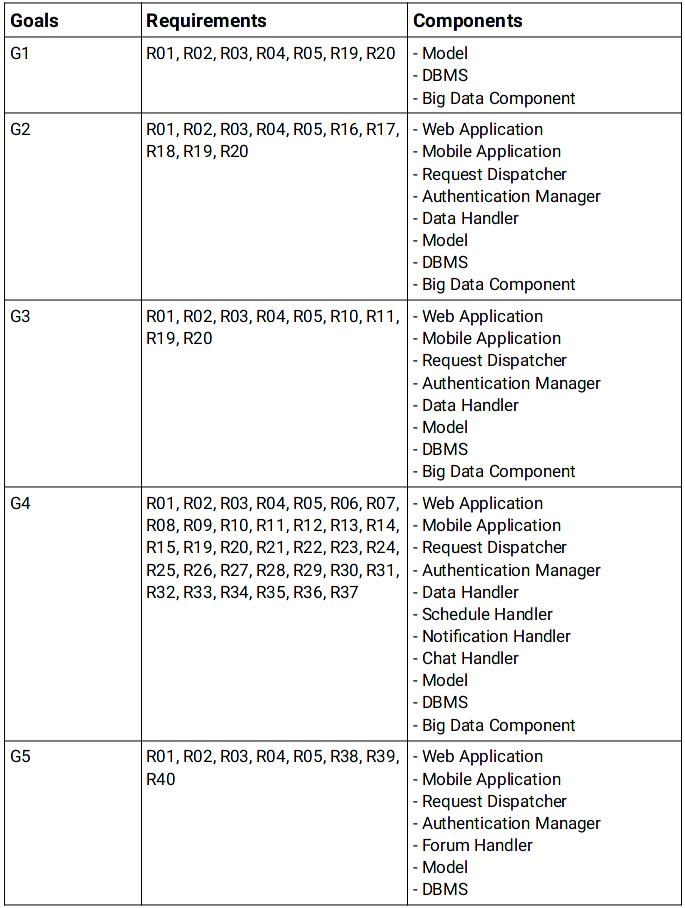
\includegraphics[width=300px]{Matrix/Matrix.jpg}
    \caption{Requirements Traceability Matrix}
\end{figure}

Notice that the component defined as "Big Data Component" denotes the set of all the components described in the section 2.3 Big-Data Tier.

\chapter{Implementation, Integration, and Unit Testing}
\section{Implementation and Integration Plan}
The system is organized as follows:
\begin{itemize}
    \item Client: it consists in the mobile application and the administrator application
    \item Web Server
    \item Application Server
    \item Internal Database
    \item Big Data Component
\end{itemize}
We will focus on the application server that contains most of the logic of the software to be. 
The strategy used for implementing and testing our software will be a bottom-up approach.
This will lead to an easier implementation as we start by coding the most basic components
and the possibility of their parallel integration.
All components will be unit tested as soon as they are implemented.\\ \\
Since there is a clear hierarchy in the structure of the software to be, some components have
an higher priority than others: this leads the process of implementation and integration.
For example, most of the components described in the Component diagram, interact
with the Model that is the bridge between the DBMS and the
Application Server.\\
The first step is to implement the Model, which is the
component that implements all methods that allow access to the Database and
perform queries and updates on it.
After that, we can proceed with the implementation and testing of the components following this order:

\begin{enumerate}
    \item \textbf{Authentication Manager}
    \item \textbf{Data Handler}
    \item \textbf{Notification Handler}
    \item \textbf{Schedule Handler}
    \item \textbf{Chat Handler}
    \item \textbf{Forum Handler}
    \item \textbf{Administration Manager}
    \item \textbf{Request Dispatcher}
\end{enumerate}

Since we are following a bottom up approach, we will use drivers to test the integration of the components,
as it can be seen from the following diagrams:
\\
\begin{figure}[H]
    \centering
    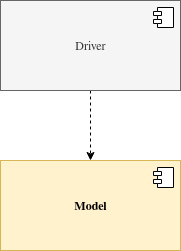
\includegraphics[width=75px]{Testing/T_01.jpg}
    \caption{Testing: Model implementation and testing}
\end{figure}

\begin{figure}[H]
    \centering
    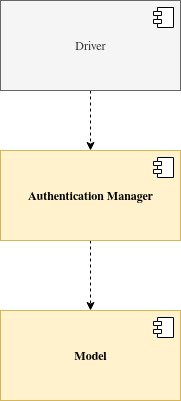
\includegraphics[width=75px]{Testing/T_02.jpg}
    \caption{Testing: Authentication Manager implementation and testing}
\end{figure}

\begin{figure}[H]
    \centering
    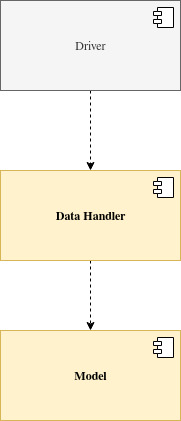
\includegraphics[width=75px]{Testing/T_03.jpg}
    \caption{Testing: Data Handler implementation and testing}
\end{figure}

\begin{figure}[H]
    \centering
    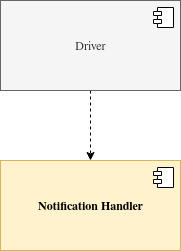
\includegraphics[width=75px]{Testing/T_04.jpg}
    \caption{Testing: Notification Handler implementation and testing}
\end{figure}

\begin{figure}[H]
    \centering
    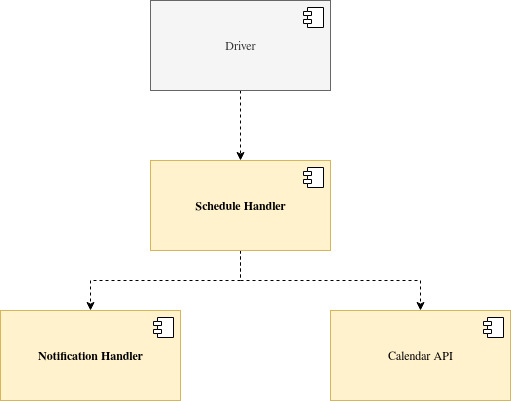
\includegraphics[width=200px]{Testing/T_05.jpg}
    \caption{Testing: Schedule Handler implementation and testing}
\end{figure}

\begin{figure}[H]
    \centering
    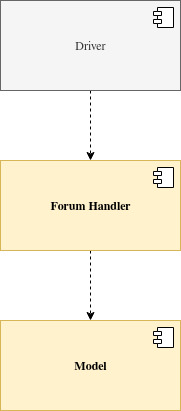
\includegraphics[width=75px]{Testing/T_06.jpg}
    \caption{Testing: Chat Handler implementation and testing}
\end{figure}

\begin{figure}[H]
    \centering
    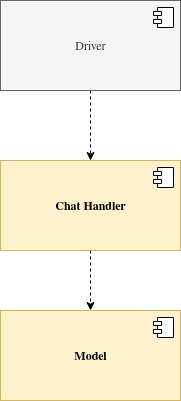
\includegraphics[width=75px]{Testing/T_07.jpg}
    \caption{Testing: Forum Handler implementation and testing}
\end{figure}

\begin{figure}[H]
    \centering
    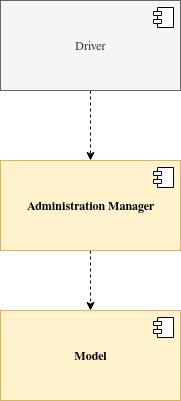
\includegraphics[width=75px]{Testing/T_08.jpg}
    \caption{Testing: Administration Manager implementation and testing}
\end{figure}

\begin{figure}[H]
    \centering
    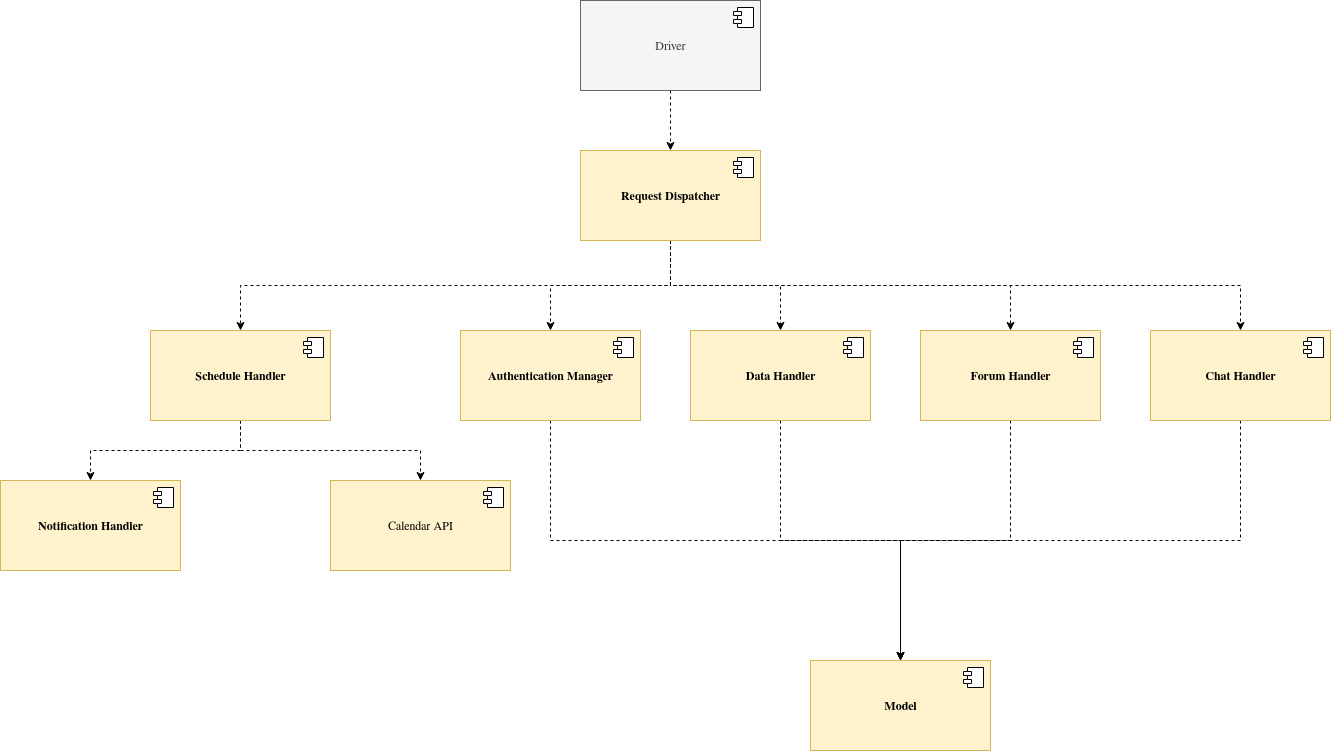
\includegraphics[width=400px]{Testing/T_09.jpg}
    \caption{Testing: Request Dispatcher implementation and testing}
\end{figure}

\section{System Testing}
Once we have integrated the components, we can start the system testing. In particular,
we need to verify that functional and non-functional requirements hold.\\ \\Moreover, the system
should go under the three main kind of testing that is:
\begin{itemize}
    \item  \textbf{Performance testing} to identify bottlenecks and possible algorithm
optimization
    \item \textbf{Load testing} helps find bugs and memory leaks
    \item  \textbf{Stress testing} to observe the resilience of the entire system under heavy
load.
\end{itemize}
All the tests in general are fundamental for studying the behavior of the
system. \\ \\ The load testing
allows developers to observe if the system could support all the many interactions made by the thousands of customers that could use the application.\\ \\
Stress testing is important because it stimulates the possible hardware and software failures procured by faulty hardware and tests the ability of the system to recover from them.\\ \\
All the system testing needs to emulate an environment as close as possible to the production environment.
\section{Acceptance Testing}
After the previously described testing, we would perform user acceptance testing. In fact, even if we verified that functional and non-functional requirements hold, we still need the acceptance from the client.\\
The test is performed following a black-box approach and typically involves users interacting with the system with actions in line with what would occur in real-time scenarios. This can verify whether the software meets all the specifications that the client wanted in the first place.
\chapter{Effort Spent}
\begin{table}[H]
\centering
\begin{tabular}{|l|l|}
\hline
\textbf{Student}       & \textbf{Effort} \\ \hline
Salvatore Maccarrone   & 30h             \\ \hline
Massimiliano Pellizzer & 30h             \\ \hline
Andrea Prati           & 40h             \\ \hline
\end{tabular}
\end{table}
\end{document}
